% ============================================================================
\section{Resultados}

A continuación se presentan los hallazgos completos del estudio en orden lógico: primero la limpieza de la base histórica del BCRP, luego los patrones estadísticos de las revisiones, después la competencia predictiva mes a mes entre los doce modelos, seguida por las simulaciones artificiales, la verificación de la regla económica y las pruebas estadísticas conjuntas finales. Por disponibilidad de librerías en el entorno de cálculo, los árboles potenciados (GBDT) se construyeron con árboles de decisión acotados en Python y el reservorio cuántico (QRC) mediante simulación exacta de cinco qubits sin ruido físico.

\subsection{Limpieza y verificación del archivo histórico}
\label{subsec:auditoria_preliminar}

La Tabla~\ref{tab:auditoria} resume los resultados de revisar de punta a punta la base histórica del BCRP recopilada por \textcite{cruz2025}. Se eliminaron filas repetidas, se comprobó que ningún dato de años futuros apareciera antes de tiempo y se verificó qué sectores tienen historia completa.

\begin{table}[htbp]
	\centering
	\caption{Auditoría de datos: resultados verificados del archivo histórico}
	\label{tab:auditoria}
	\footnotesize
	\renewcommand{\arraystretch}{1.15}
	\begin{tabular}{@{}>{\raggedright\arraybackslash}p{5.2cm}>{\raggedright\arraybackslash}p{2.3cm}>{\raggedright\arraybackslash}p{6.0cm}@{}}
		\toprule
		Indicador de auditoría & Valor & Estado / evidencia\\
		\midrule
		Registros sector--boletín & 44\,307 & Verificado en tabla consolidada\\
		Actividades económicas & 9 & Verificado (cobertura desigual por sector)\\
		Boletines mensuales continuos & 1994-01 a 2025-12 & Verificado (384 meses sin faltantes en PBI)\\
		Meses económicos cubiertos & 1992-01 a 2025-10 & Verificado (406 meses)\\
		Períodos PBI limpios a \(H=11\) & 350 (374 brutos) & Verificado; 0 huecos internos (1993-10 a 2024-11)\\
		Períodos PBI limpios a \(H=12\) & 331 (355 brutos) & Verificado; 18 huecos internos (diciembres 2018--2023 y 2015--2016)\\
		Períodos excluidos en \(H=11\) & 56 & 21 sin primer dato oportuno + 11 fin de muestra + 24 cambio de año base\\
		Detalle de fechas & Mensual & Aproximación mensual en tiempo real (sin día exacto)\\
		Sectores con serie continua & 6 de 9 & Servicios desde 1997-07; electricidad desde 2003-05; minería omite 9 meses (2018--2019)\\
		Duplicados y fuga futura & Resuelto (0 fugas) & 3\,131 filas repetidas eliminadas; 0 datos adelantados\\
		\bottomrule
	\end{tabular}
	\fuente{elaboración propia a partir del repositorio histórico del BCRP \parencite{cruz2025}.}
\end{table}

La Figura~\ref{fig:triangulo} muestra cómo cambian las estimaciones del PBI desde su primera publicación hasta doce meses después. Allí se observan claramente dos saltos bruscos que corresponden a los cambios de año base oficiales (julio de 2000 y marzo de 2014), además de pequeños vacíos en la línea de doce meses debido al formato de publicación de las Notas Semanales. Esa observación confirma por qué conviene usar el plazo de once meses (\(H=11\)) como serie principal continua y dejar doce, seis y tres meses como verificación adicional.

\begin{figure}[htbp]
	\centering
	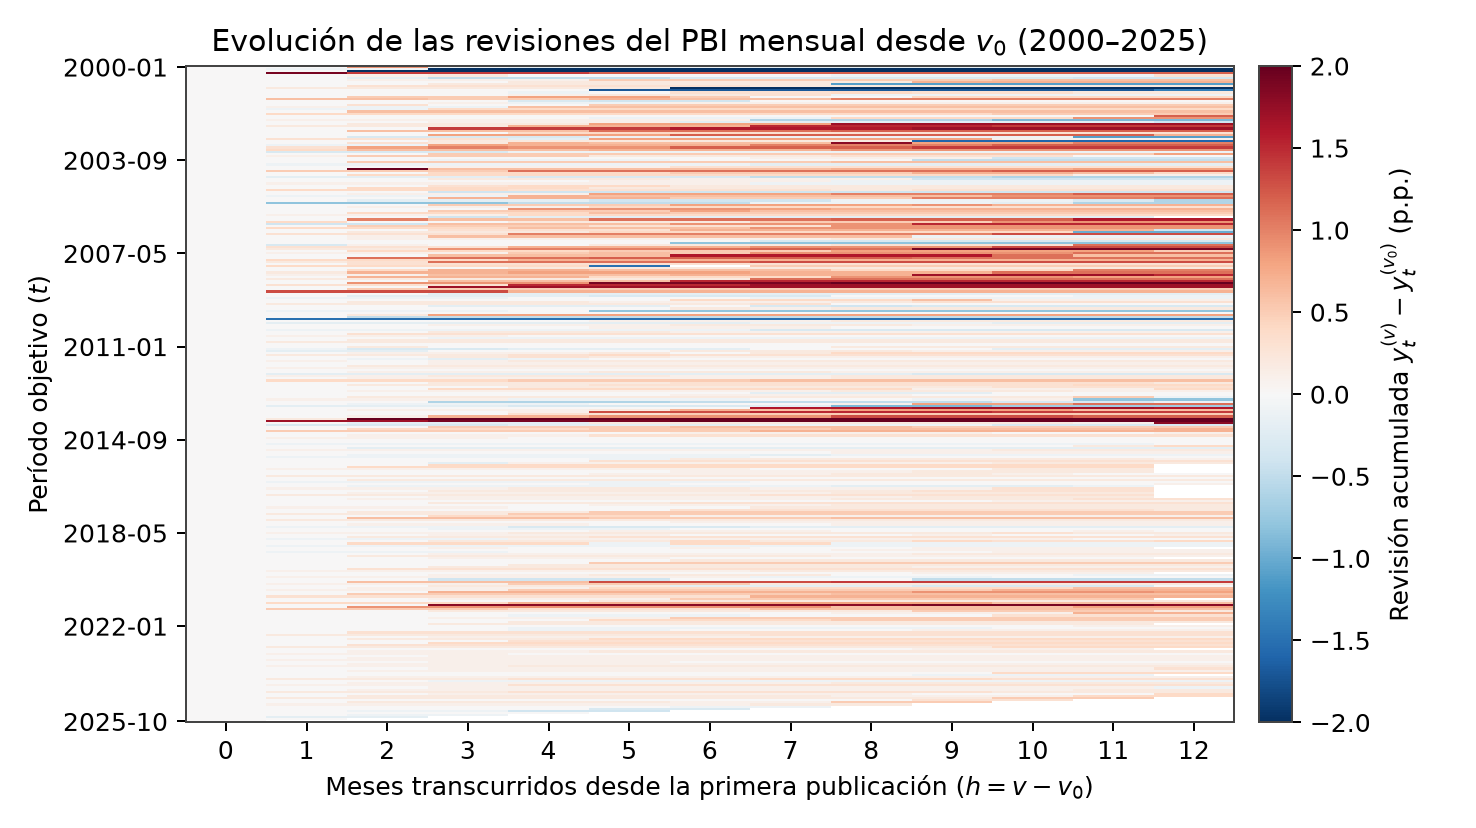
\includegraphics[width=0.92\textwidth]{images/triangulo_gdp.png}
	\caption{Evolución de las revisiones acumuladas del PBI mensual desde la primera publicación \(v_0\) (2000--2025)}
	\label{fig:triangulo}
	\fuente{elaboración propia a partir de los registros históricos del BCRP.}
\end{figure}

\subsection{Comportamiento básico de las revisiones}
\label{subsec:descriptivos}

El hallazgo principal al comparar cifras preliminares con sus versiones corregidas es directo: \textbf{cuando se publica por primera vez el PBI mensual del Perú, suele quedarse corto}. Como muestra la Tabla~\ref{tab:descriptivos_revision}, once meses después (\(H=11\)) la tasa corregida sube en promedio \(+0{,}347\) puntos porcentuales respecto al primer anuncio (y \(+0{,}363\) puntos si se mide a doce meses). La misma tendencia al alza aparece en todos los horizontes evaluados, desde tres meses (\(+0{,}205\) puntos) hasta la comparación con el último dato disponible (\(+0{,}256\) puntos, equivalente con signo invertido al \(-0{,}256\) visto en la lectura inicial; Anexo~\ref{app:objetivo}).

\begin{table}[htbp]
	\centering
	\caption{Estadísticos descriptivos de la revisión del PBI (\(y_t^{(v_H)} - y_t^{(v_0)}\)) según horizonte y depuración}
	\label{tab:descriptivos_revision}
	\footnotesize
	\setlength{\tabcolsep}{4.5pt}
	\renewcommand{\arraystretch}{1.15}
	\begin{tabular}{@{}l S[table-format=3.0] S[table-format=-1.3] S[table-format=1.3] S[table-format=-1.3] S[table-format=-1.3] S[table-format=-1.3] S[table-format=-1.3] S[table-format=1.3]@{}}
		\toprule
		Muestra / horizonte & {$n$} & {Media} & {DE} & {Mín.} & {P25} & {Mediana} & {P75} & {Máx.}\\
		\midrule
		\(H=11\) limpio (principal) & 350 & 0.347 & 0.768 & -2.000 & 0.000 & 0.200 & 0.600 & 4.900\\
		\(H=11\) bruto (con base) & 374 & 0.305 & 0.930 & -5.500 & 0.000 & 0.200 & 0.600 & 4.900\\
		\(H=12\) limpio (sensibilidad) & 331 & 0.363 & 0.798 & -2.000 & 0.000 & 0.200 & 0.700 & 4.900\\
		\(H=6\) limpio (sensibilidad) & 355 & 0.311 & 0.598 & -2.000 & 0.000 & 0.200 & 0.500 & 4.000\\
		\(H=3\) limpio (sensibilidad) & 358 & 0.205 & 0.452 & -1.500 & 0.000 & 0.100 & 0.300 & 2.500\\
		Horizonte variable (última \(-\) primera) & 406 & 0.256 & 0.930 & -5.500 & 0.000 & 0.200 & 0.600 & 4.200\\
		\bottomrule
	\end{tabular}
	\fuente{elaboración propia a partir de la muestra depurada de publicaciones del BCRP.}
\end{table}

La Tabla~\ref{tab:descriptivos_revision} también demuestra la utilidad de retirar los \(24\) meses afectados por cambios de año base: al separarlos, desaparece la caída extrema de \(-5{,}500\) puntos (quedando en \(-2{,}000\)) y la dispersión baja de \(0{,}930\) a \(0{,}768\), señal de que esos grandes saltos negativos reflejaban empalmes estadísticos y no correcciones corrientes. Por su parte, la demora habitual para publicar por primera vez un mes se mantuvo prácticamente fija en dos meses (promedio de \(2{,}003\) meses).

Las Figuras~\ref{fig:scatter}, \ref{fig:hist} y~\ref{fig:horizontes} ilustran visualmente estos rasgos: la relación casi uno a uno pero ligeramente desplazada hacia arriba entre primera y última cifra, la distribución concentrada a la derecha del cero tras separar cambios de base, y cómo cae la cantidad de datos útiles al alargar demasiado el horizonte (cayendo a \(5\) observaciones en \(18\) meses y a \(0\) en \(24\) meses).

\begin{figure}[htbp]
	\centering
	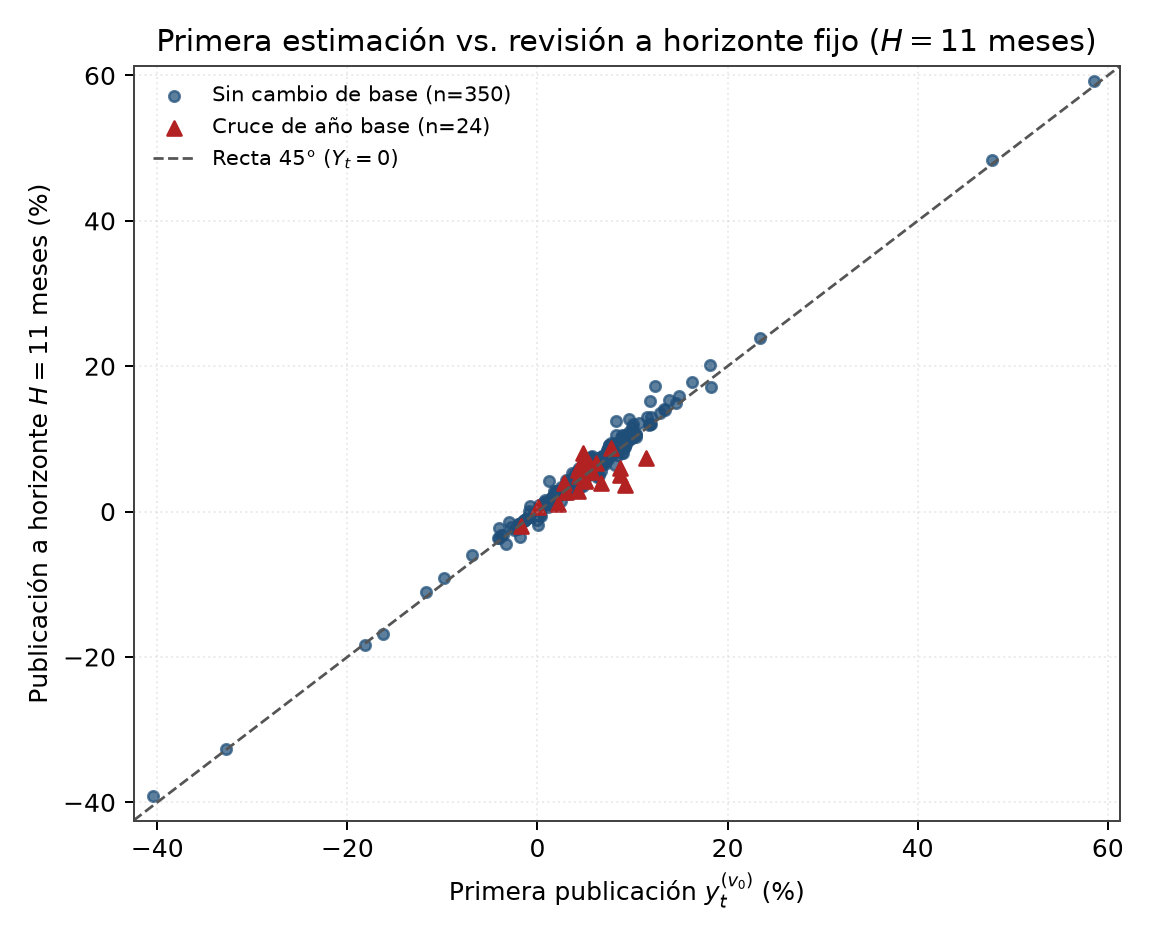
\includegraphics[width=0.72\textwidth]{images/scatter_revisiones_gdp.png}
	\caption{Primera publicación \(y_t^{(v_0)}\) frente a publicación a horizonte fijo \(H=11\) meses}
	\label{fig:scatter}
	\fuente{elaboración propia.}
\end{figure}

\begin{figure}[htbp]
	\centering
	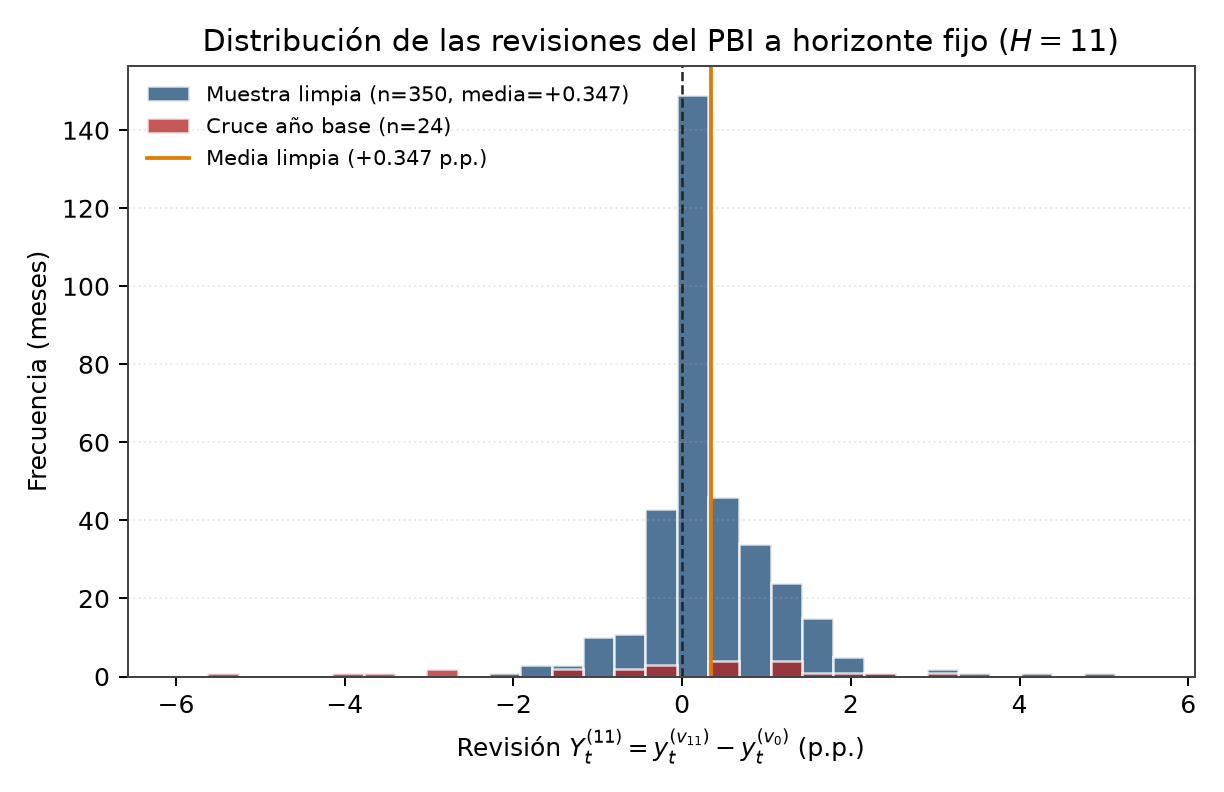
\includegraphics[width=0.76\textwidth]{images/hist_revisiones_gdp.png}
	\caption{Distribución de la revisión \(Y_t^{(11)} = y_t^{(v_{11})} - y_t^{(v_0)}\) con separación de cambios de año base}
	\label{fig:hist}
	\fuente{elaboración propia.}
\end{figure}

\begin{figure}[htbp]
	\centering
	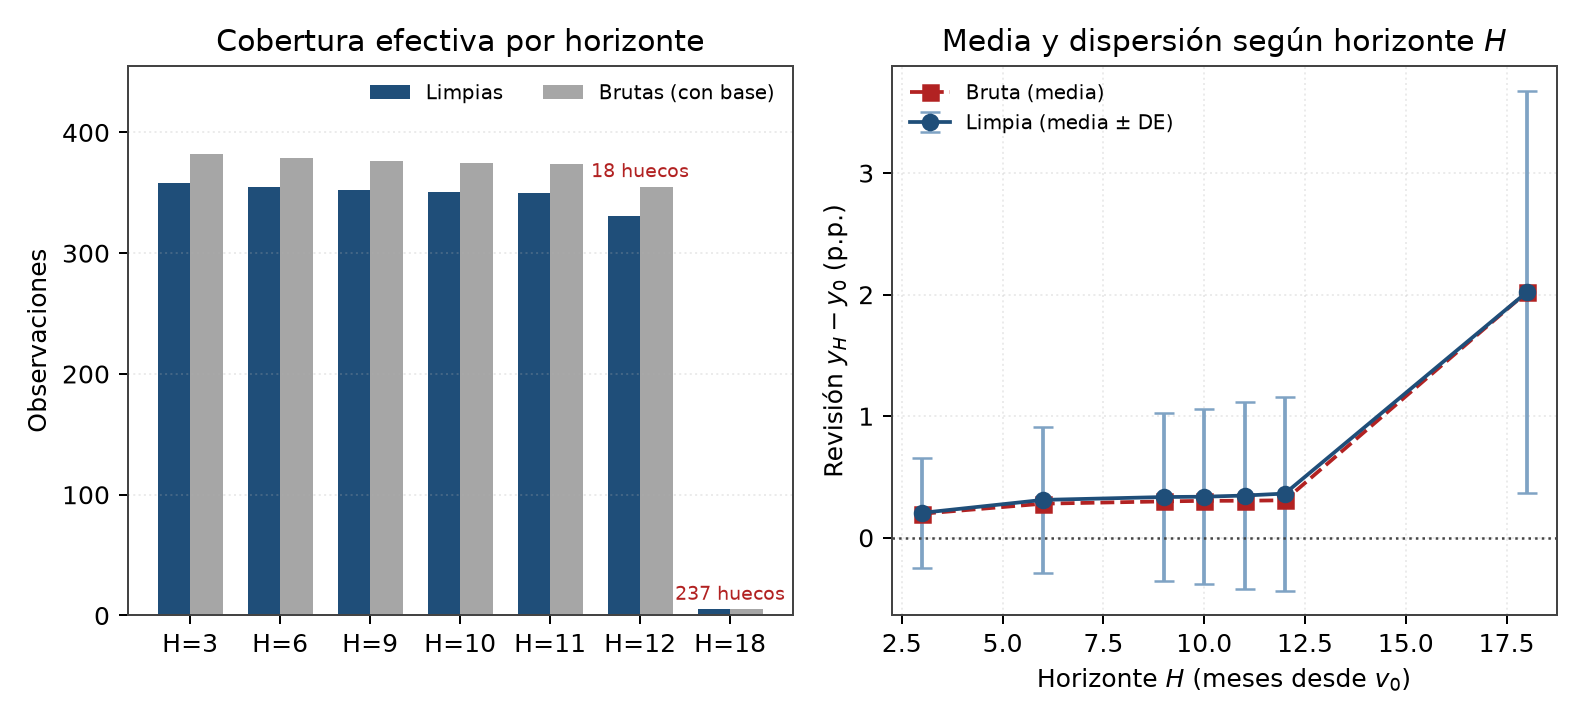
\includegraphics[width=0.92\textwidth]{images/metricas_horizonte_gdp.png}
	\caption{Cobertura efectiva y media/desviación estándar de las revisiones según horizonte \(H\)}
	\label{fig:horizontes}
	\fuente{elaboración propia.}
\end{figure}

\subsection{Qué patrones estadísticos siguen las revisiones}
\label{subsec:econometria}

Antes de entrenar modelos complejos, se verificó si las revisiones seguían reglas observables o si eran puro ruido. Las pruebas tomaron en cuenta que los errores de meses cercanos se parecen entre sí aplicando la corrección de \textcite{newey1987} (tanto en su versión estándar como considerando once meses de solapamiento).

\paragraph{Sesgo constante hacia arriba y valores extremos poco comunes.}
En todos los plazos evaluados (\(3\), \(6\), \(11\) y \(12\) meses), el promedio positivo es altamente significativo (\(p < 10^{-5}\); Tabla~\ref{tab:etapa2_sesgo}), descartando que se trate de coincidencia. Además, aparecen revisiones grandes positivas con más frecuencia de lo que tendría una campana normal (asimetría positiva y curtosis elevada, prueba de normalidad rechazada con \(p < 10^{-100}\)), razón por la cual las simulaciones posteriores incluyeron sacudidas no normales.

\begin{table}[htbp]
	\centering
	\caption{Pruebas estadísticas de sesgo medio y distribución en muestras limpias}
	\label{tab:etapa2_sesgo}
	\footnotesize
	\renewcommand{\arraystretch}{1.15}
	\begin{tabular}{@{}l S[table-format=3.0] S[table-format=1.3] S[table-format=1.3] l S[table-format=1.3] l S[table-format=1.3] S[table-format=1.3] S[table-format=3.1]@{}}
		\toprule
		Horizonte & {$n$} & {Media} & {$\text{SE}_{\text{NW}}$} & {\(p_{\text{NW}}\)} & {$\text{SE}_{\text{solap}}$} & {\(p_{\text{solap}}\)} & {Asim.} & {Curt.\ exc.} & {JB}\\
		\midrule
		\(H=3\)  & 358 & 0.205 & 0.033 & \(<10^{-9}\) & 0.031 & \(<10^{-10}\) & 1.394 & 5.736 & 589.4\\
		\(H=6\)  & 355 & 0.311 & 0.047 & \(<10^{-10}\) & 0.049 & \(<10^{-9}\)  & 1.163 & 6.523 & 687.9\\
		\(H=11\) & 350 & 0.347 & 0.064 & \(5{,}3\times 10^{-8}\) & 0.075 & \(3{,}6\times 10^{-6}\) & 1.258 & 6.293 & 649.6\\
		\(H=12\) & 331 & 0.363 & 0.067 & \(5{,}7\times 10^{-8}\) & 0.080 & \(5{,}6\times 10^{-6}\) & 1.145 & 5.465 & 468.6\\
		\bottomrule
	\end{tabular}
	\fuente{elaboración propia a partir de las pruebas econométricas sobre la muestra depurada. Todos los estadísticos Jarque--Bera arrojan \(p < 10^{-100}\).}
\end{table}

\paragraph{Un ciclo anual repetitivo y diferencias por mes.}
La Figura~\ref{fig:acf_estac} revela un detalle práctico clave para pronosticar en tiempo real: aunque las revisiones de meses inmediatos están fuertemente conectadas entre sí (\(\hat{\rho}_1 = +0{,}453\); \cite{ljung1978} \(p = 1{,}4\times 10^{-41}\)), esas revisiones recientes todavía no terminan cuando nace un dato nuevo. En cambio, las revisiones que sí ya terminaron \textbf{un año atrás} conservan una relación clara con el mes actual (correlación anual de \(+0{,}386\) en el mes doce, \(p=1{,}3\times 10^{-12}\)). A esto se suma un patrón estacional marcado: el primer trimestre del año recibe las mayores correcciones hacia arriba (enero \(+0{,}731\), febrero \(+0{,}503\) y marzo \(+0{,}734\) puntos), mientras noviembre (\(+0{,}143\)) y diciembre (\(-0{,}083\)) apenas cambian.

\begin{figure}[htbp]
	\centering
	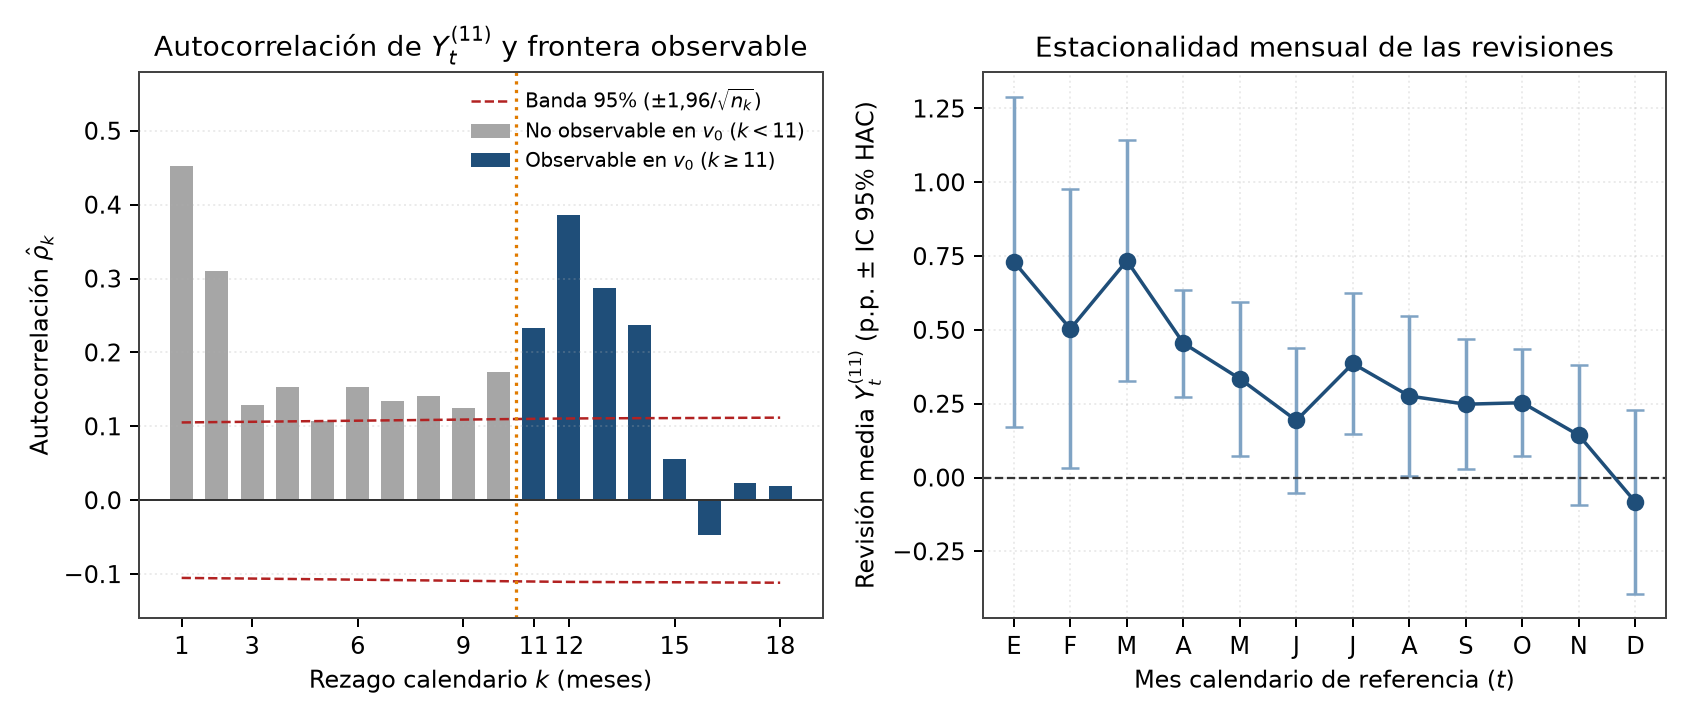
\includegraphics[width=0.95\textwidth]{images/etapa2_acf_pacf.png}
	\caption{Repetición temporal de la revisión \(Y_t^{(11)}\) respecto a la frontera observable en tiempo real (izquierda) y promedio por mes del año (derecha)}
	\label{fig:acf_estac}
	\fuente{elaboración propia a partir de la serie histórica limpia (\(n=350\)).}
\end{figure}

La Tabla~\ref{tab:etapa2_rt} comprueba cuánta variación de las revisiones se explica usando únicamente información ya disponible en el primer anuncio (\(n=313\)). Los dos rezagos anuales completados explican por sí solos un \(15{,}7\%\) (\(R^2 = 0{,}1569\)), y al juntarlos con el dato preliminar, cambios recientes ya publicados y el mes del año se alcanza un \(22{,}3\%\) (\(R^2 = 0{,}2225\), \(p = 2{,}6\times 10^{-7}\)). Este resultado confirma la Hipótesis~1: las revisiones del PBI tienen una señal real predecible.

\begin{table}[htbp]
	\centering
	\caption{Capacidad explicativa usando únicamente información observable en \(v_0(t)\) (\(n=313\))}
	\label{tab:etapa2_rt}
	\footnotesize
	\renewcommand{\arraystretch}{1.15}
	\begin{tabular}{@{}l c S[table-format=1.4] S[table-format=1.4] S[table-format=1.3] l S[table-format=3.2]@{}}
		\toprule
		Información observable en \(v_0(t)\) & Variables & {\(R^2\)} & {\(\bar{R}^2\)} & {\(F_{\text{NW}}\)} & {\(p\)-valor HAC} & {BIC}\\
		\midrule
		Solo primera publicación (\(y_t^{(v_0)}\)) & 1 & 0.0230 & 0.0198 & 4.999 & \(0{,}0261\) & 677.59\\
		Revisiones de hace 1 año (\(Y_{t-11}, Y_{t-12}\)) & 2 & 0.1569 & 0.1515 & 9.197 & \(1{,}3\times 10^{-4}\) & 637.20\\
		Revisiones recientes observables (\(s=1,2\)) & 2 & 0.0179 & 0.0115 & 4.120 & \(0{,}0171\) & 684.97\\
		Mes del año (estacionalidad) & 11 & 0.0807 & 0.0471 & 2.249 & \(0{,}0122\) & 716.00\\
		Modelo conjunto observable en \(v_0\) & 16 & 0.2225 & 0.1804 & 4.190 & \(2{,}6\times 10^{-7}\) & 692.30\\
		\bottomrule
	\end{tabular}
	\fuente{elaboración propia con base en las estimaciones en tiempo real del estudio.}
\end{table}

\paragraph{Estabilidad por épocas, efecto de la pandemia y diferencias entre sectores.}
Al comprobar mediante la prueba de \textcite{mincer1969} si la primera cifra refleja toda la información sin sesgo (Tabla~\ref{tab:etapa2_mz}), en todas las épocas se rechaza la eficiencia perfecta debido principalmente al empuje constante hacia arriba (\(\hat{\alpha} > 0\)). Al revisar qué cambió con los años (Figura~\ref{fig:regimenes}), sobresalen dos hechos muy importantes:
\begin{enumerate}
	\item \textbf{La variabilidad bajó antes de la pandemia:} entre 1993 y 2012 las revisiones oscilaban bastante (desviación estándar de \(1{,}289\) y \(0{,}716\)), pero entre 2014 y 2019 la serie se volvió muy estable (\(\text{DE}=0{,}196\)), aunque mantuvo su sesgo positivo de \(+0{,}163\) puntos \parencite{engle1982}.
	\item \textbf{Las relaciones curvas aparecen solo por la pandemia:} aunque la prueba de linealidad de \textcite{ramsey1969} marca señal no lineal en la serie completa (\(p=0{,}0010\)), al mirar época por época se descubre que antes de 2020 una relación recta funcionaba perfectamente bien (2000--2012 \(p=0{,}9112\); 2014--2019 \(p=0{,}2085\)). La curvatura aparece únicamente entre 2020 y 2024 (\(p=0{,}0003\)), motivando analizar los modelos antes y después del COVID-19 por separado.
\end{enumerate}

\begin{table}[htbp]
	\centering
	\caption{Pruebas de eficiencia (\(y_t^{(v_H)} = \alpha + \beta y_t^{(v_0)} + u_t\)) y diagnósticos por época}
	\label{tab:etapa2_mz}
	\footnotesize
	\setlength{\tabcolsep}{4pt}
	\renewcommand{\arraystretch}{1.15}
	\begin{tabular}{@{}l S[table-format=3.0] S[table-format=1.3] S[table-format=1.3] S[table-format=1.3] S[table-format=1.3] S[table-format=2.2] l l l@{}}
		\toprule
		Muestra / época & {$n$} & {\(\hat{\alpha}\)} & {\(\text{SE}_{\alpha}\)} & {\(\hat{\beta}\)} & {\(\text{SE}_{\beta}\)} & {\(F_{\text{Wald}}\)} & {\(p_{\text{Wald}}\)} & {\(p_{\text{ARCH}}\)} & {\(p_{\text{RESET}}\)}\\
		\midrule
		Limpia \(H=11\) (global) & 350 & 0.273 & 0.064 & 1.018 & 0.010 & 16.23 & \(1{,}8\times 10^{-7}\) & \(3{,}1\times 10^{-7}\) & \(0{,}0010\)\\
		Limpia \(H=12\) (global) & 331 & 0.297 & 0.067 & 1.016 & 0.009 & 15.84 & \(2{,}7\times 10^{-7}\) & \(1{,}2\times 10^{-6}\) & \(0{,}0048\)\\
		Limpia \(H=6\) (global)  & 355 & 0.270 & 0.051 & 1.010 & 0.007 & 23.35 & \(3{,}0\times 10^{-10}\) & \(5{,}5\times 10^{-6}\) & \(0{,}0038\)\\
		Limpia \(H=3\) (global)  & 358 & 0.172 & 0.032 & 1.008 & 0.005 & 20.70 & \(3{,}1\times 10^{-9}\) & \(9{,}6\times 10^{-6}\) & \(0{,}1283\)\\
		\midrule
		1993-10 a 1999-04 (Base 90/94) & 67 & 0.356 & 0.245 & 1.052 & 0.041 & 4.69 & \(0{,}0125\) & \(0{,}4572\) & \(0{,}0514\)\\
		2000-06 a 2012-12 (Base 94)    & 151 & 0.054 & 0.129 & 1.052 & 0.022 & 10.42 & \(5{,}8\times 10^{-5}\) & \(0{,}0407\) & \(0{,}9112\)\\
		2014-02 a 2019-12 (Pre-COVID)  & 71 & 0.180 & 0.047 & 0.994 & 0.012 & 16.96 & \(1{,}0\times 10^{-6}\) & \(0{,}0231\) & \(0{,}2085\)\\
		2020-01 a 2024-11 (COVID+)     & 59 & 0.297 & 0.057 & 1.004 & 0.006 & 13.95 & \(1{,}2\times 10^{-5}\) & \(0{,}5904\) & \(0{,}0003\)\\
		\bottomrule
	\end{tabular}
	\fuente{elaboración propia con ajuste de errores estándar HAC (\(L_{\text{NW}}\)).}
\end{table}

\begin{figure}[htbp]
	\centering
	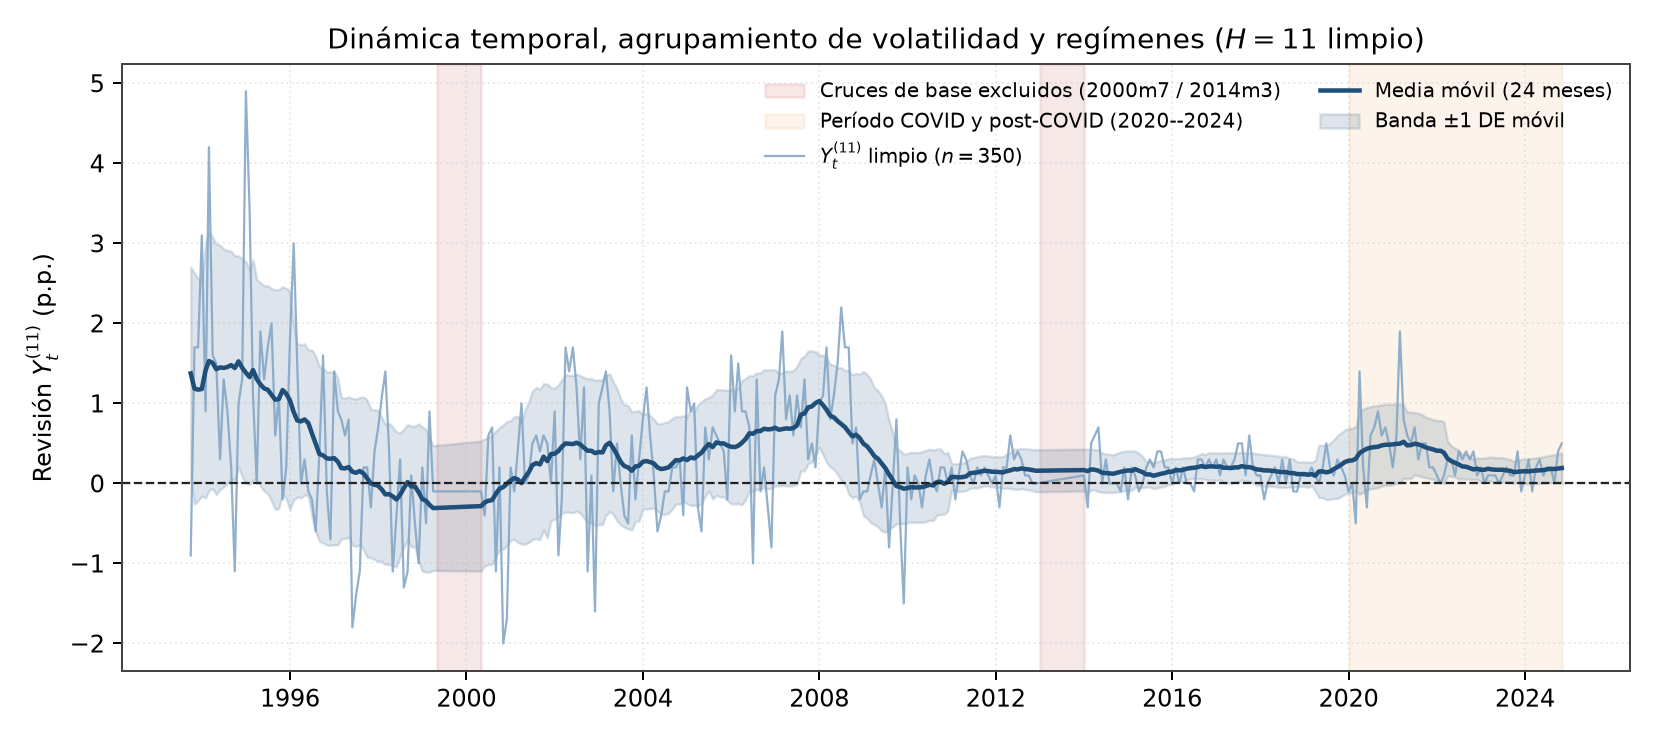
\includegraphics[width=0.95\textwidth]{images/etapa2_regimenes_evolucion.png}
	\caption{Evolución temporal de \(Y_t^{(11)}\), promedio y dispersión móviles por épocas económicas (1993--2024)}
	\label{fig:regimenes}
	\fuente{elaboración propia a partir de la serie limpia del PBI peruano.}
\end{figure}

Por último, la Figura~\ref{fig:sectores} muestra que las correcciones al alza no ocurren por igual en toda la economía: se concentran en pesca (\(+2{,}143\) puntos), agropecuario (\(+0{,}821\)), comercio (\(+0{,}562\)), manufactura (\(+0{,}525\)) y minería (\(+0{,}505\)), sectores donde es más difícil reunir cifras completas el primer mes. En cambio, construcción (\(+0{,}098\)), servicios (\(+0{,}076\)) y electricidad (\(-0{,}011\)) casi no se corrigen en promedio.

\begin{figure}[htbp]
	\centering
	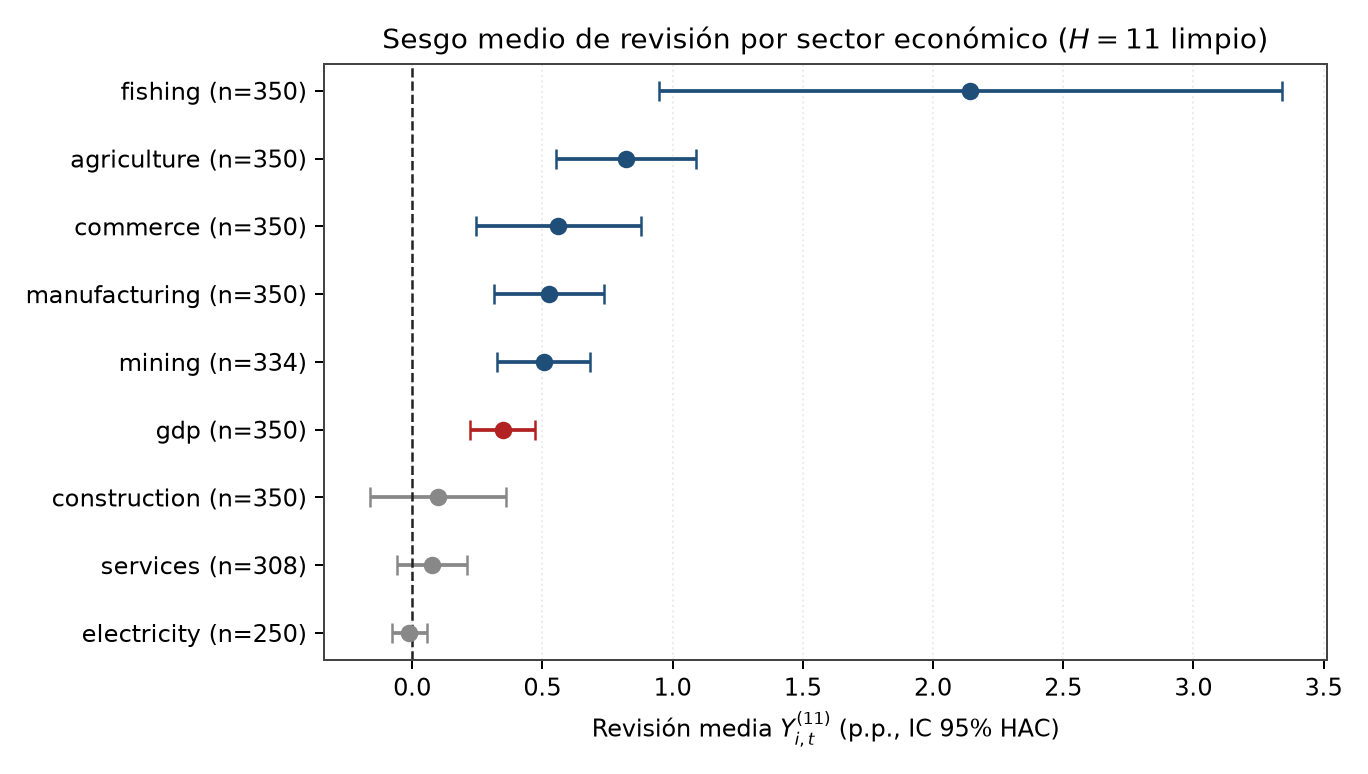
\includegraphics[width=0.82\textwidth]{images/etapa2_sectores_sesgo.png}
	\caption{Sesgo medio de revisión por sector económico a horizonte \(H=11\) limpio (intervalo de confianza al 95\%)}
	\label{fig:sectores}
	\fuente{elaboración propia con base en las series sectoriales verificadas.}
\end{figure}

\subsection{Desempeño de los modelos prediciendo mes a mes}
\label{subsec:desempeno_modelos}

Para probar qué modelo predice mejor en condiciones reales, los doce competidores emitieron pronósticos mes a mes durante más de veinte años: \(250\) fechas entre febrero de 2003 y noviembre de 2024. En cada mes solo se entrenaron con el historial ya cerrado hasta ese día, manteniendo aparte los últimos \(60\) meses (diciembre de 2019 a noviembre de 2024) para el examen final. De forma automática dentro del pasado, el modelo autorregresivo eligió casi siempre mirar los dos años anteriores (\(99{,}2\%\) de las veces) y Ridge aplicó una regularización alta (\(\lambda=500\)) para equilibrar las variables sectoriales.

La Tabla~\ref{tab:metricas} resume los errores globales de todo el período, y la Tabla~\ref{tab:etapa3_regimenes} separa lo ocurrido antes de la pandemia y durante los últimos cinco años. En la lectura global, \textbf{el menor error correspondió a las características aleatorias de Fourier (RFF, \(\text{RMSE}=0{,}456\))}, seguidas por la red clásica ESN de veinte neuronas (\(\text{RMSE}=0{,}472\)) y recién en tercer lugar por el modelo cuántico QRC (\(\text{RMSE}=0{,}478\)).

\begin{table}[htbp]
	\centering
	\caption{Desempeño predictivo global de los doce modelos sobre \(Y_t^{(11)}\) (2003m2--2024m11, \(n=250\))}
	\label{tab:metricas}
	\footnotesize
	\renewcommand{\arraystretch}{1.15}
	\begin{tabular}{@{}>{\raggedright\arraybackslash}p{4.5cm}S[table-format=1.3]S[table-format=1.3]S[table-format=-1.3]S[table-format=-1.3]l@{}}
		\toprule
		Modelo & {RMSE} & {MAE} & {Sesgo} & {$R^2_{\text{OOS}}$} & {IC 95\% \(\Delta\text{RMSE}\) (vs. Ridge)}\\
		\midrule
		Referencia nula (\(\widehat{Y}=0\)) & 0.574 & 0.396 & 0.292 & -0.349 & {\([-0{,}135;\; +0{,}150]\), \(p_{\text{DM}}=0{,}918\)}\\
		Corrección de sesgo (media exp.) & 0.513 & 0.395 & -0.131 & -0.077 & {\([-0{,}176;\; +0{,}057]\), \(p_{\text{DM}}=0{,}430\)}\\
		Corrección de sesgo (móvil 60m) & 0.525 & 0.381 & 0.021 & -0.127 & {\([-0{,}164;\; +0{,}064]\), \(p_{\text{DM}}=0{,}512\)}\\
		Autorregresivo AR (BIC) & 0.498 & 0.356 & -0.037 & -0.016 & {\([-0{,}189;\; +0{,}044]\), \(p_{\text{DM}}=0{,}301\)}\\
		ARX observable (BIC) & 0.558 & 0.384 & -0.015 & -0.276 & {\([-0{,}068;\; +0{,}037]\), \(p_{\text{DM}}=0{,}791\)}\\
		Regresión Ridge (benchmark, 20 var.) & 0.566 & 0.384 & -0.064 & -0.312 & {Referencia principal (\(0{,}000\))}\\
		Factores dinámicos (DFM + Ridge) & 0.605 & 0.392 & -0.067 & -0.498 & {\([-0{,}001;\; +0{,}086]\), \(p_{\text{DM}}=0{,}184\)}\\
		Árboles potenciados (GBDT)\textsuperscript{a} & 0.495 & 0.356 & -0.068 & -0.003 & {\([-0{,}193;\; +0{,}032]\), \(p_{\text{DM}}=0{,}290\)}\\
		Características aleatorias (RFF, \(m=20\))\textsuperscript{b} & 0.456 & 0.334 & -0.069 & 0.149 & {\([-0{,}222;\; -0{,}013]\), \(p_{\text{DM}}=0{,}094\)}\\
		Reservorio clásico ESN (20 n.)\textsuperscript{b} & 0.472 & 0.341 & -0.057 & 0.087 & {\([-0{,}188;\; -0{,}004]\), \(p_{\text{DM}}=0{,}103\)}\\
		Reservorio clásico ESN (64 n.)\textsuperscript{b} & 0.508 & 0.379 & -0.038 & -0.056 & {\([-0{,}136;\; +0{,}014]\), \(p_{\text{DM}}=0{,}200\)}\\
		Reservorio cuántico QRC (5 qubits)\textsuperscript{b} & 0.478 & 0.352 & -0.102 & 0.063 & {\([-0{,}208;\; +0{,}020]\), \(p_{\text{DM}}=0{,}196\)}\\
		\bottomrule
	\end{tabular}
	\caption*{\footnotesize \textit{Nota:} \textsuperscript{a}Árboles CART acotados (\texttt{GBDT\_NumPy} en gráficos). \textsuperscript{b}Promedios deterministas sobre cinco semillas (\texttt{101, 202, 303, 404, 505}); \texttt{QRC\_Ising5} usa simulación exacta por matriz densidad. Intervalos bootstrap por bloques \parencite{politis1992} (\(L=12\), \(B=2000\)); valor \(p_{\text{DM}}\) bilateral de \textcite{harvey1997}.}
	\fuente{elaboración propia con base en las evaluaciones fuera de muestra del estudio (2003--2024).}
\end{table}

Al separar los períodos normales de la pandemia en la Tabla~\ref{tab:etapa3_regimenes} (y las Figuras~\ref{fig:etapa3_oos}--\ref{fig:etapa4_estabilidad}), la historia queda completamente clara:
\begin{enumerate}
	\item \textbf{En épocas normales (2003--2019), la regresión Ridge funcionó bien:} antes del COVID-19, Ridge fue el mejor modelo lineal clásico (\(\text{RMSE}=0{,}503\)), superando con claridad al promedio histórico simple (\(0{,}550\), \(p=0{,}0071\)) y a los árboles de decisión (\(0{,}533\), \(p=0{,}0086\)). Incluso entre 2014 y 2019 el simple promedio móvil de sesenta meses logró \(\text{RMSE}=0{,}210\) con sesgo casi nulo.
	\item \textbf{Durante la pandemia (2020--2024), las fórmulas lineales se dispararon y los modelos acotados evitaron el error:} en abril de 2020 la primera cifra del PBI cayó \(-40{,}5\%\) y en abril de 2021 rebotó \(+58{,}5\%\). Al aplicar una recta sobre números tan extremos, Ridge predijo correcciones absurdas (\(-1{,}464\) y \(+4{,}020\) puntos porcentuales, cuando la revisión real fue \(+1{,}4\) y \(+0{,}8\)), elevando su error a \(\text{RMSE}=0{,}731\). Eso también distorsionó la prueba anidada de \textcite{clark2007} (\(\text{CW}=3{,}554\)). En cambio, los \textbf{árboles acotados (GBDT)} limitaron sus pronósticos (\(+0{,}241\) y \(+0{,}909\)) y obtuvieron el mejor desempeño del tramo final (\(\text{RMSE}=0{,}349\)), superando tanto a Ridge como a la referencia nula.
	\item \textbf{El modelo cuántico (QRC) frenó los extremos, pero no venció a los equivalentes clásicos:} gracias a que sus veinte mediciones quedan acotadas entre \(-1\) y \(+1\), QRC logró el segundo mejor error en pandemia (\(\text{RMSE}=0{,}363\)) y superó globalmente a la simple corrección por promedio histórico (\(0{,}478\) vs. \(0{,}513\), \(p=0{,}0175\)). Sin embargo, no venció a sus controles clásicos equivalentes: empató estadísticamente con ESN de veinte neuronas (\(0{,}472\), \(p=0{,}730\)) y perdió frente a RFF (\(0{,}456\), \(p=0{,}0146\) global y \(p=0{,}0038\) antes de la pandemia). Además, aumentar ESN de \(20\) a \(64\) neuronas empeoró el resultado (\(0{,}508\), \(p=0{,}046\)), probando que las series económicas cortas premian modelos compactos. También se observó que QRC varía bastante según la semilla aleatoria usada (promedio individual \(0{,}5160 \pm 0{,}0316\)), por lo que su resultado final dependió de promediar cinco ejecuciones.
\end{enumerate}

\begin{table}[htbp]
	\centering
	\caption{Desempeño antes del COVID-19 (2003m2--2019m11) frente al tramo final congelado (2019m12--2024m11)}
	\label{tab:etapa3_regimenes}
	\footnotesize
	\renewcommand{\arraystretch}{1.12}
	\begin{tabular}{@{}>{\raggedright\arraybackslash}p{4.5cm}S[table-format=1.3]S[table-format=1.3]S[table-format=-1.3]S[table-format=1.3]S[table-format=1.3]S[table-format=-1.3]@{}}
		\toprule
		& \multicolumn{3}{c}{Pre-pandemia (\(n=190\))} & \multicolumn{3}{c}{Tramo final (\(n=60\))}\\
		\cmidrule(lr){2-4}\cmidrule(lr){5-7}
		Modelo & {RMSE} & {MAE} & {$R^2_{\text{OOS}}$} & {RMSE} & {MAE} & {$R^2_{\text{OOS}}$}\\
		\midrule
		Referencia nula (\(\widehat{Y}=0\)) & 0.602 & 0.414 & -0.299 & 0.474 & 0.338 & -0.682\\
		Corrección media expansiva & 0.550 & 0.433 & -0.084 & 0.371 & 0.274 & -0.033\\
		Corrección móvil \(60\text{m}\) & 0.559 & 0.416 & -0.120 & 0.396 & 0.269 & -0.175\\
		Autorregresivo AR (BIC) & 0.526 & 0.384 & 0.007 & 0.396 & 0.267 & -0.175\\
		ARX observable (BIC) & 0.521 & 0.383 & 0.028 & 0.663 & 0.387 & -2.290\\
		Regresión Ridge (benchmark) & 0.503 & 0.375 & 0.094 & 0.731 & 0.413 & -3.001\\
		Factores dinámicos (DFM + Ridge) & 0.515 & 0.379 & 0.050 & 0.827 & 0.434 & -4.125\\
		Árboles potenciados (GBDT) & 0.533 & 0.394 & -0.017 & 0.349 & 0.237 & 0.087\\
		Características aleatorias (RFF) & 0.480 & 0.355 & 0.174 & 0.368 & 0.269 & -0.017\\
		Reservorio clásico ESN (20 n.) & 0.485 & 0.359 & 0.156 & 0.427 & 0.285 & -0.367\\
		Reservorio clásico ESN (64 n.) & 0.505 & 0.389 & 0.088 & 0.518 & 0.348 & -1.008\\
		Reservorio cuántico QRC (5 qubits) & 0.509 & 0.379 & 0.070 & 0.363 & 0.266 & 0.013\\
		\bottomrule
	\end{tabular}
	\fuente{elaboración propia con base en los resultados fuera de muestra por épocas (2003--2024).}
\end{table}

En síntesis, la capacidad de contener choques como los de 2020--2021 provino simplemente del acotamiento no lineal de las variables, y no de una ventaja propia de la mecánica cuántica (las pruebas numéricas previas confirmaron asimismo fidelidad física exacta del simulador, con errores inferiores a \(10^{-14}\), y cero uso de datos futuros).

\begin{figure}[htbp]
	\centering
	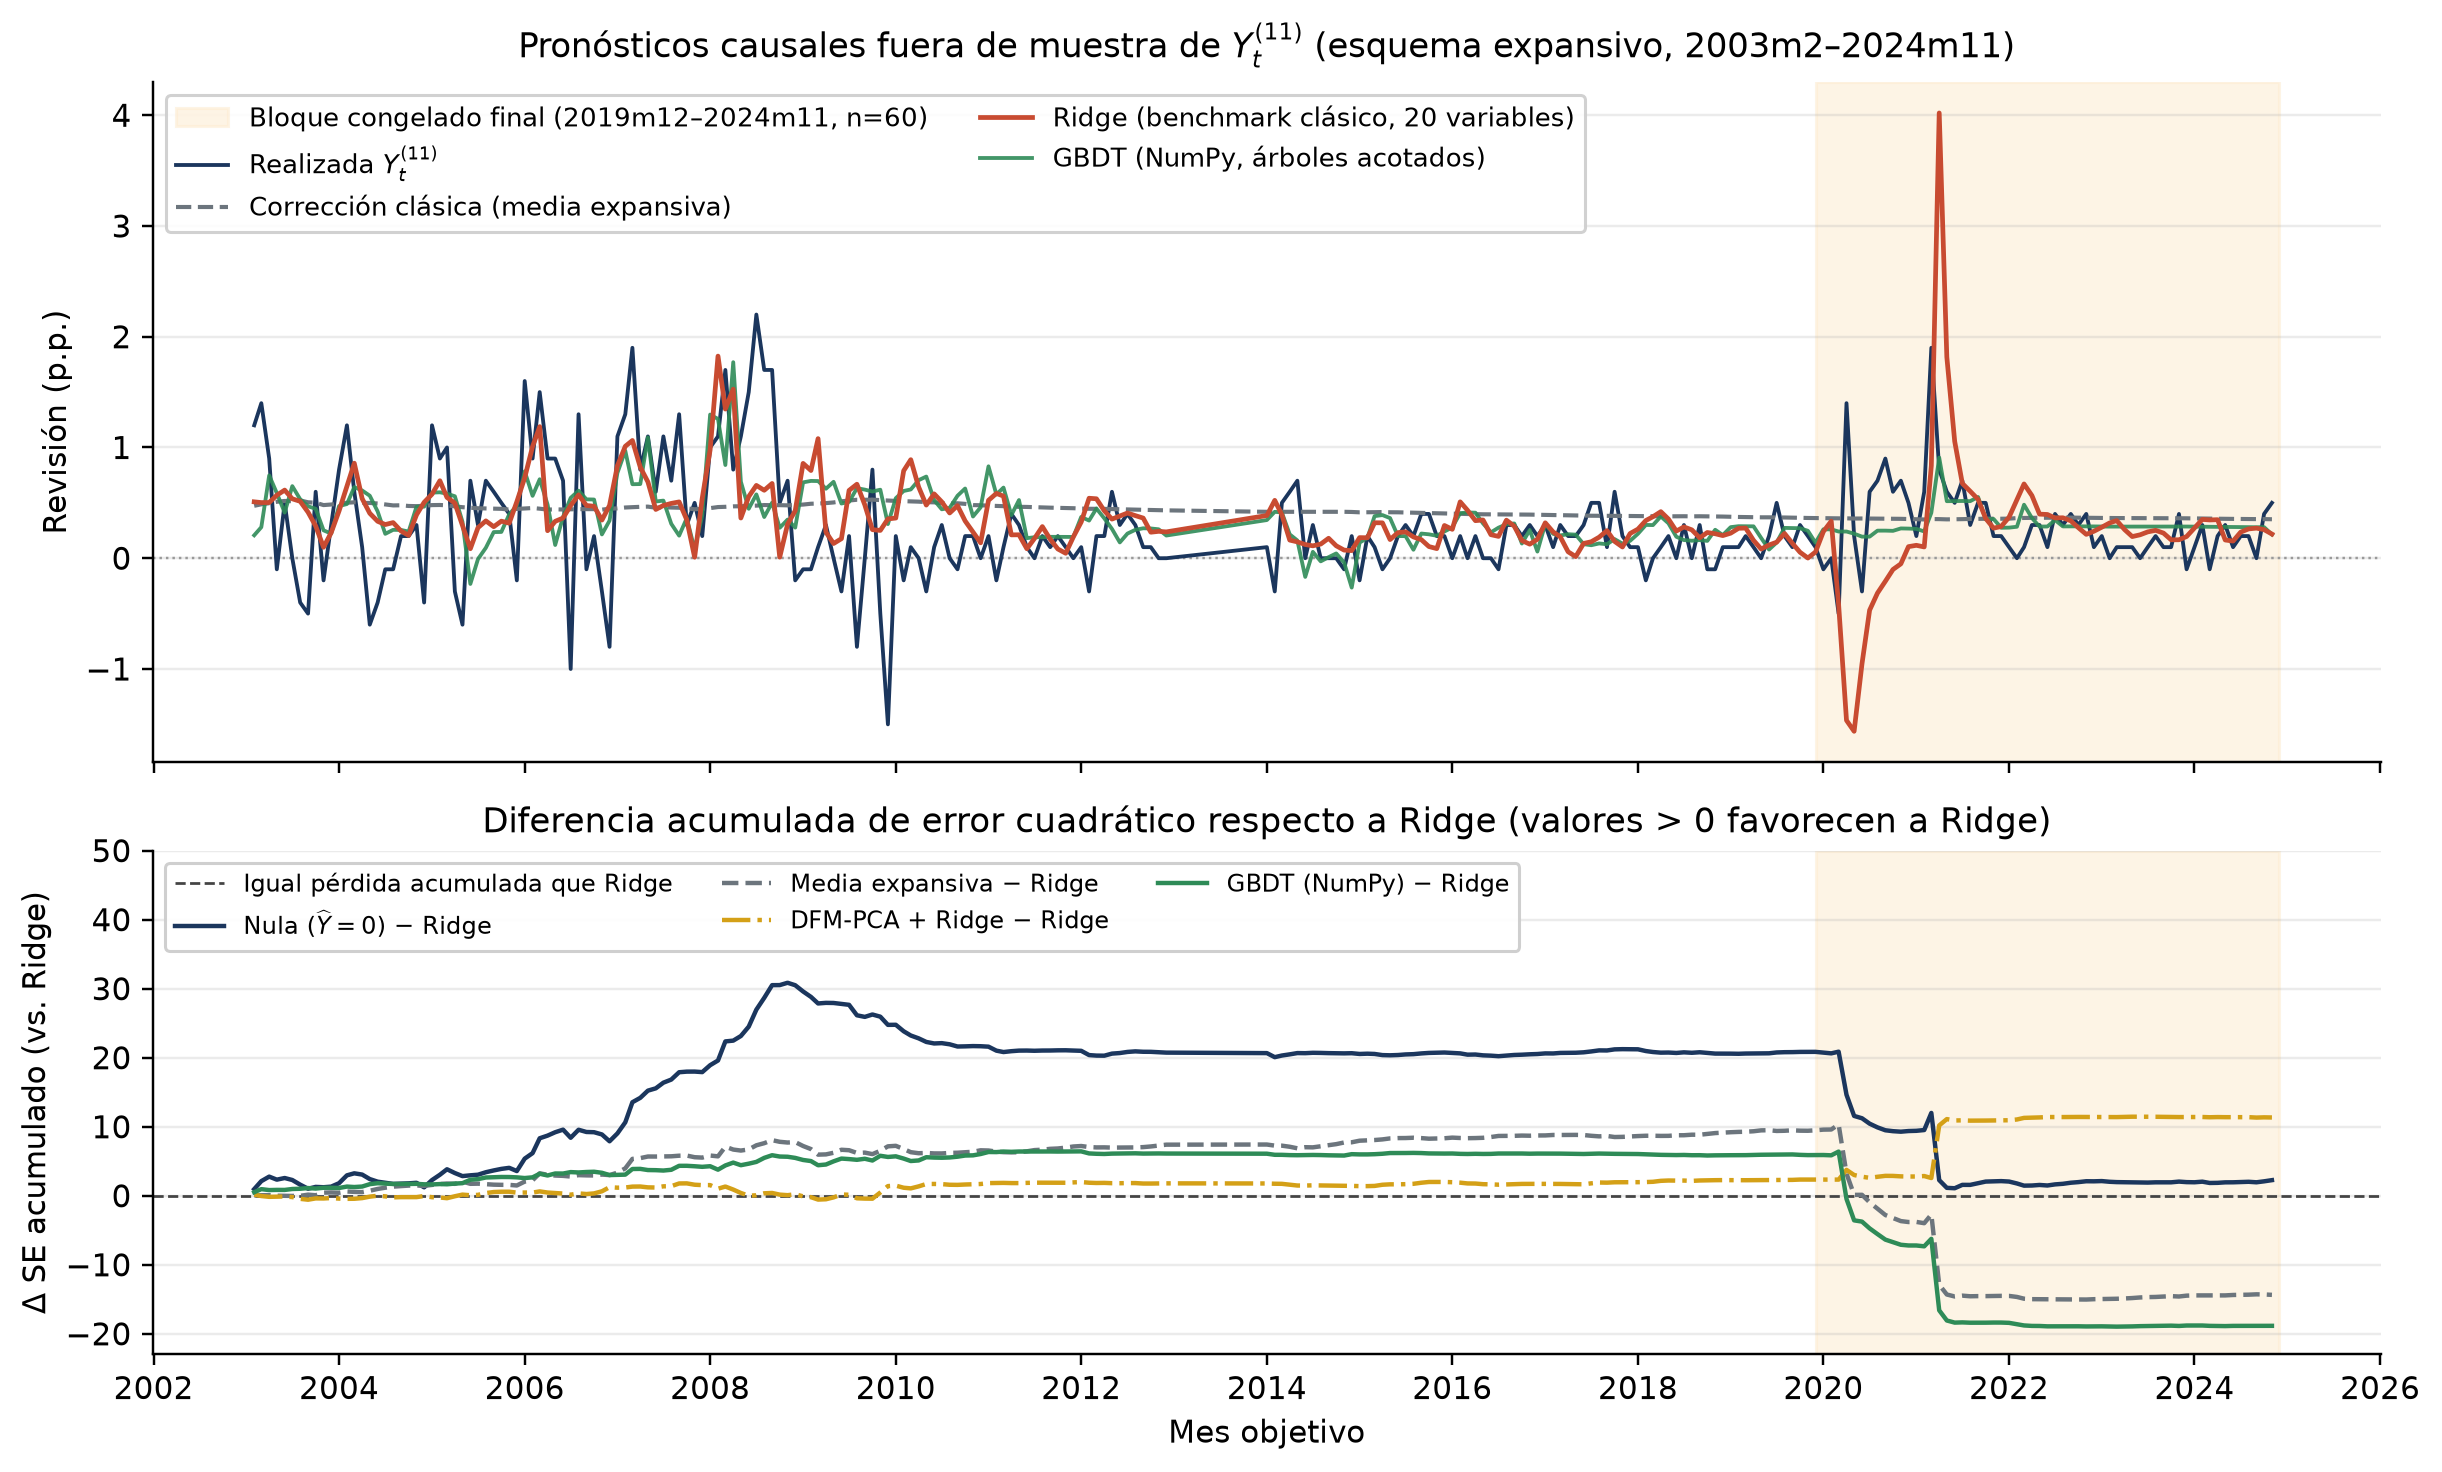
\includegraphics[width=0.96\textwidth]{images/etapa3_oos_predicciones.png}
	\caption{Pronósticos mensuales en tiempo real de modelos clásicos (arriba) y error acumulado frente a Ridge (abajo), 2003m2--2024m11.}
	\label{fig:etapa3_oos}
\end{figure}

\begin{figure}[htbp]
	\centering
	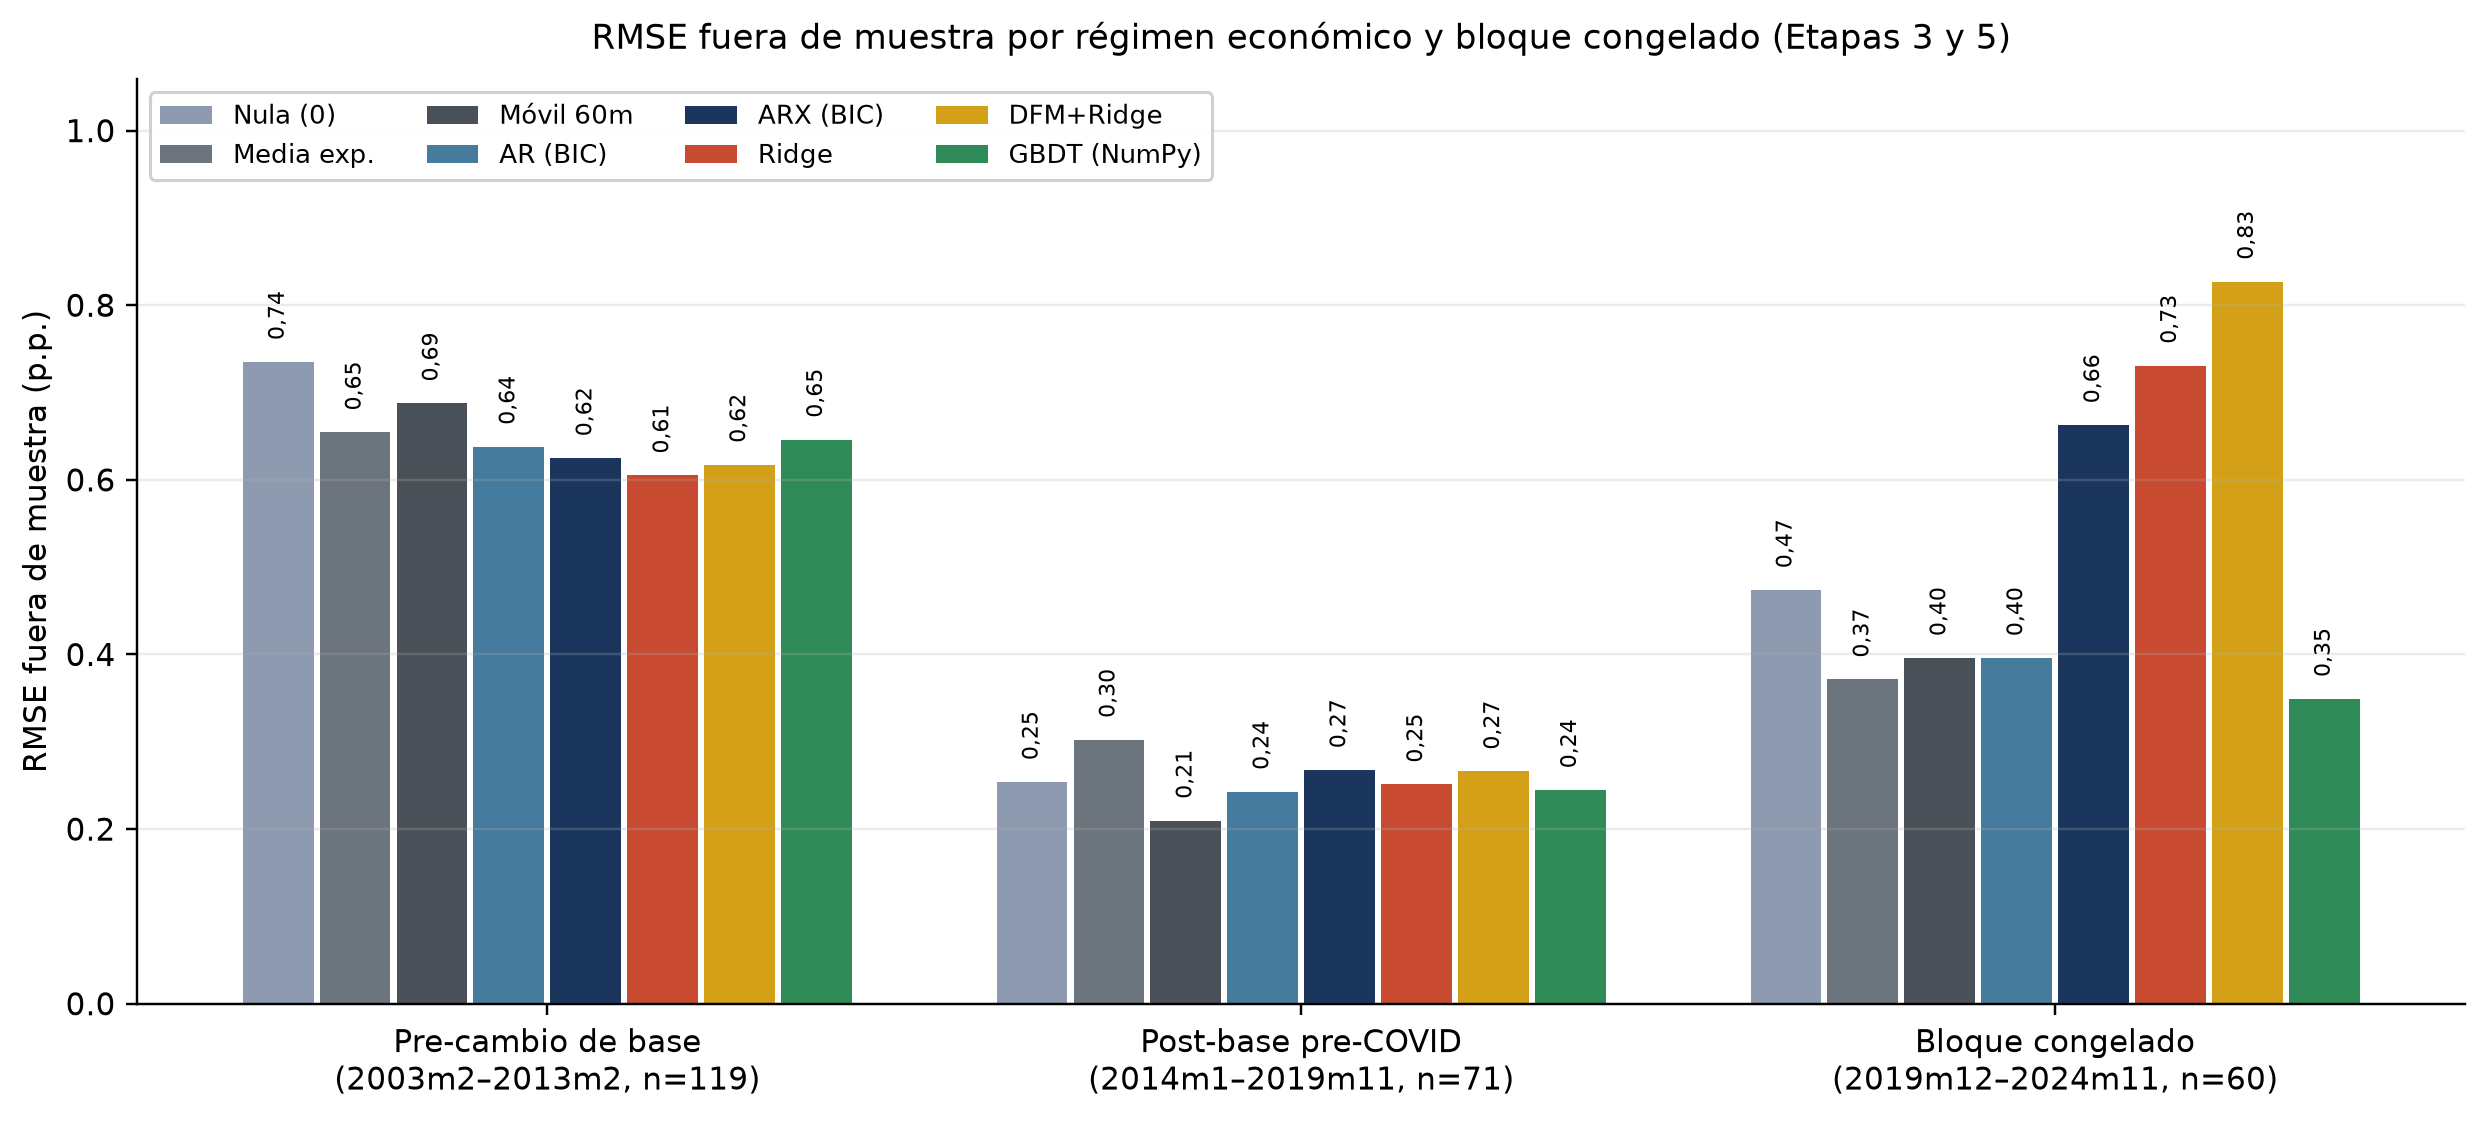
\includegraphics[width=0.96\textwidth]{images/etapa3_rmse_regimenes.png}
	\caption{Error RMSE por época económica y tramo final para los ocho referentes clásicos.}
	\label{fig:etapa3_regimenes}
\end{figure}

\begin{figure}[htbp]
	\centering
	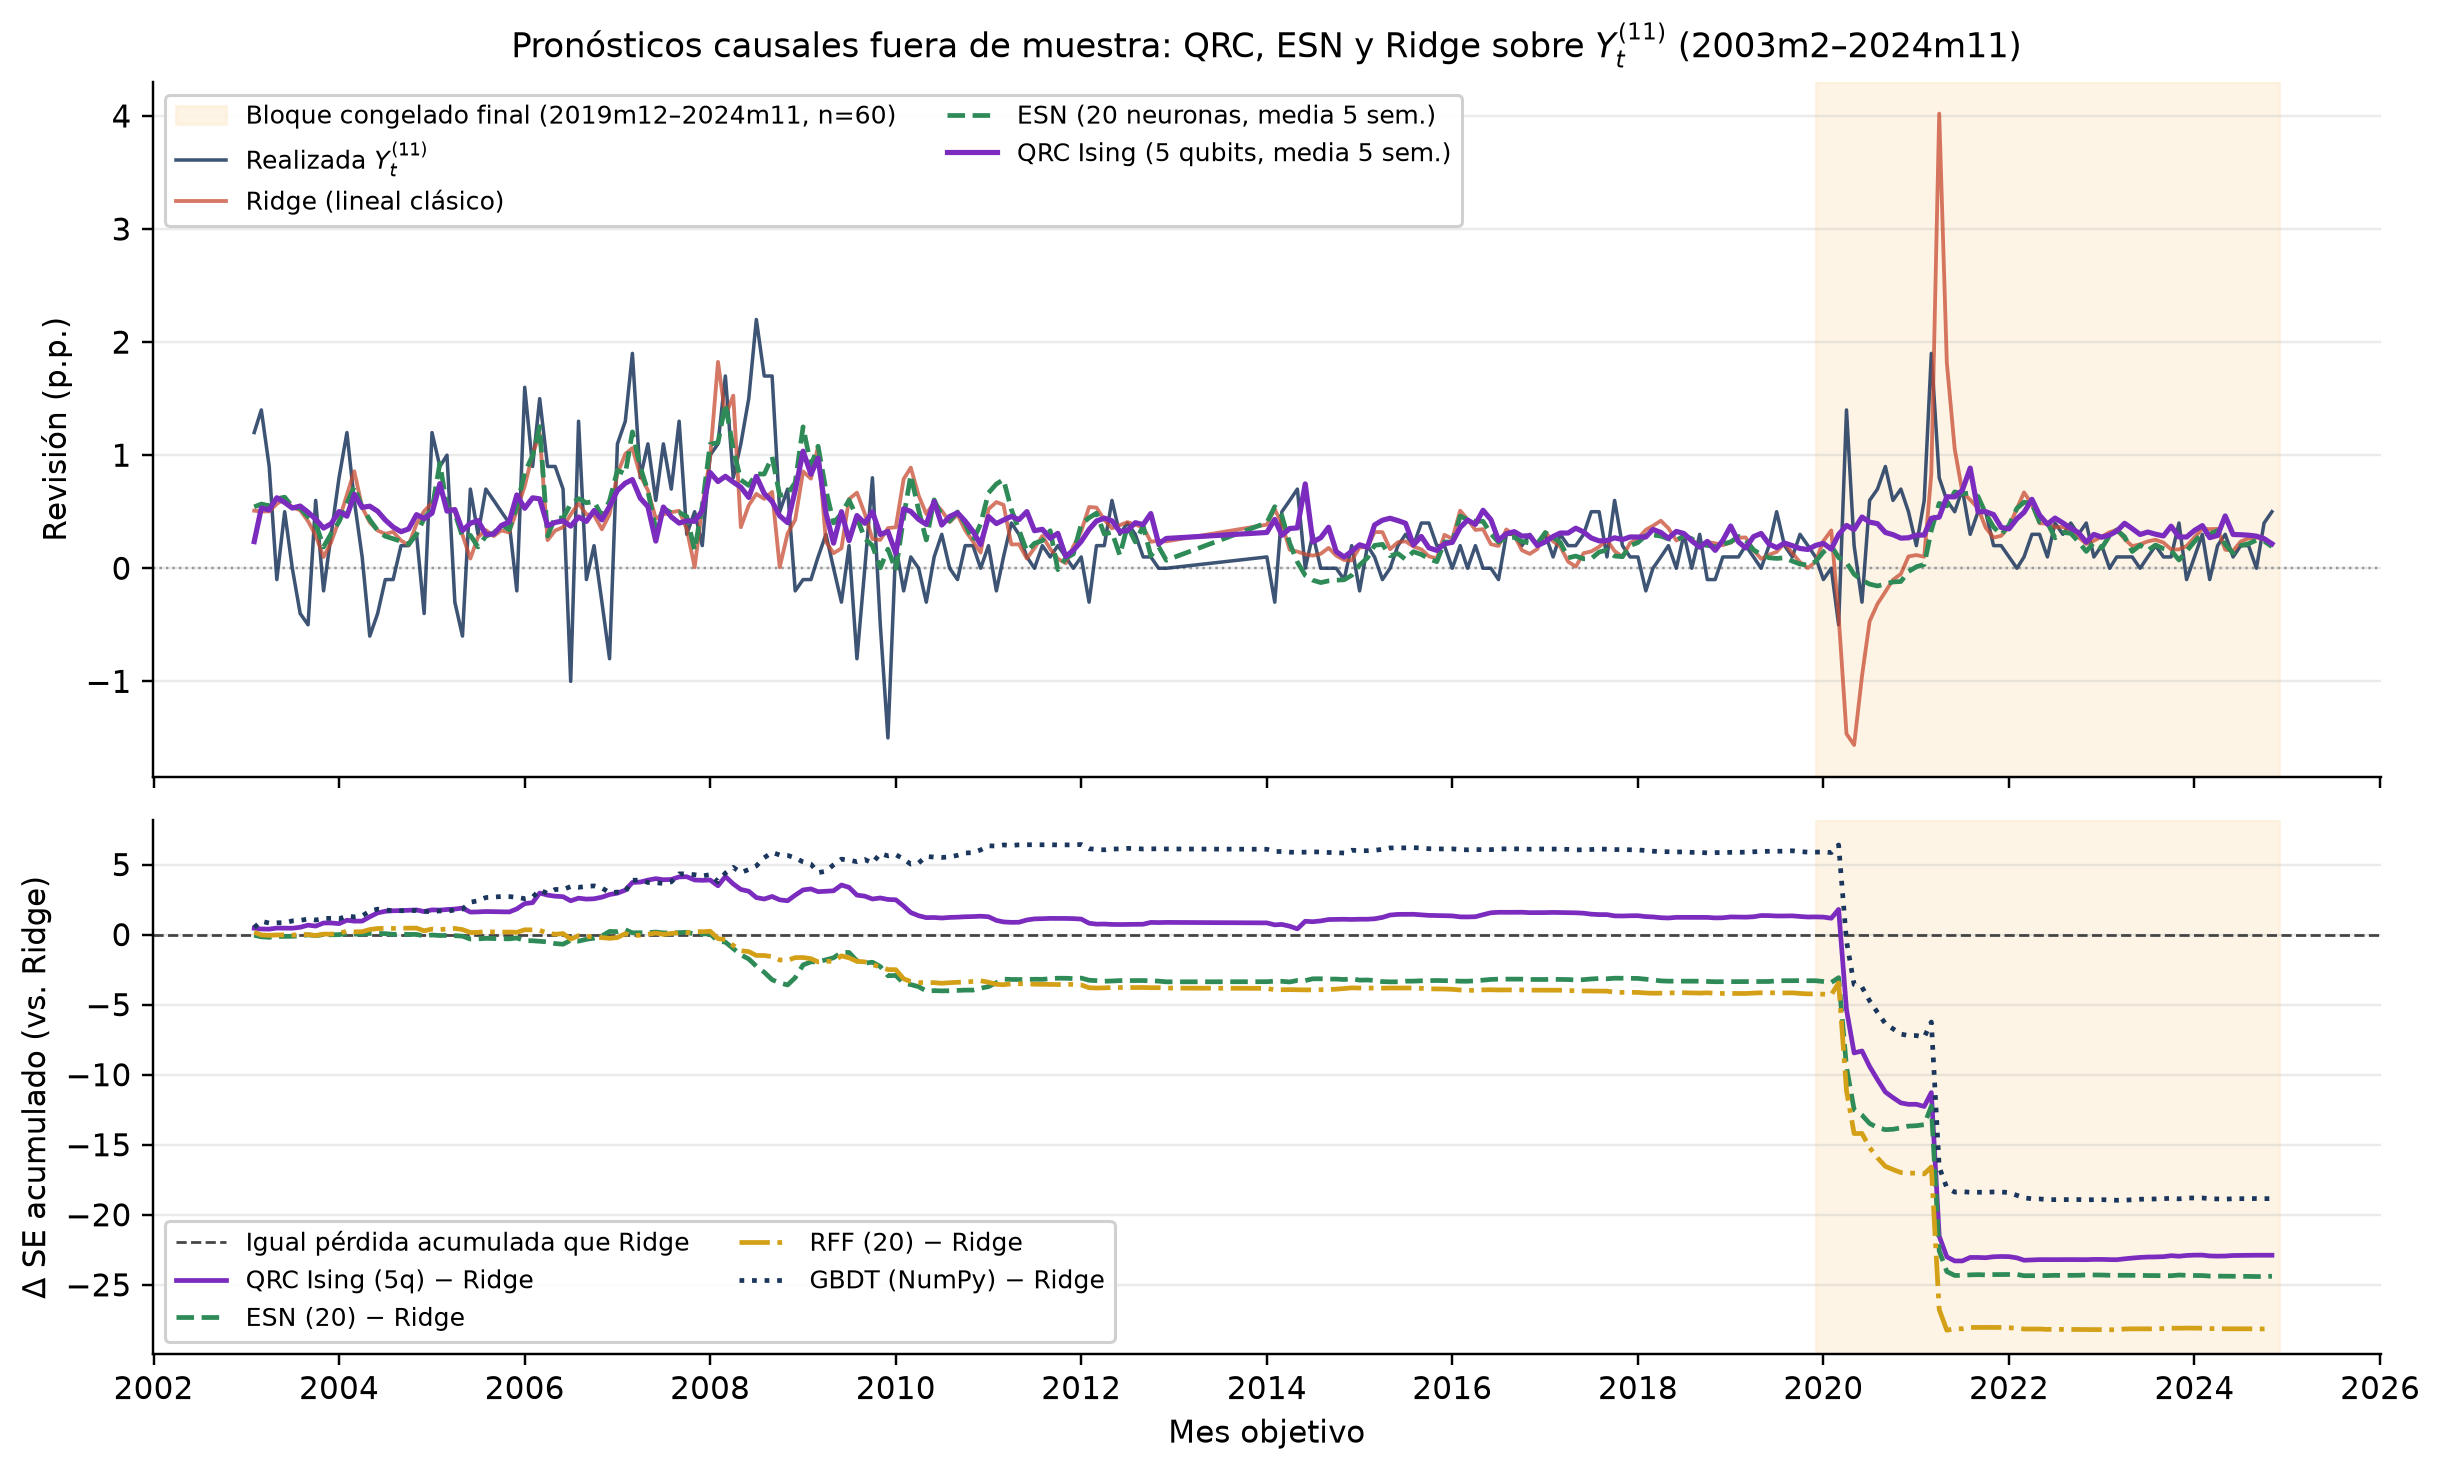
\includegraphics[width=0.96\textwidth]{images/etapa4_reservorios_oos.png}
	\caption{Pronósticos en tiempo real (arriba) y pérdida acumulada frente a Ridge (abajo) para QRC, ESN, RFF y GBDT (2003m2--2024m11).}
	\label{fig:etapa4_oos}
\end{figure}

\begin{figure}[htbp]
	\centering
	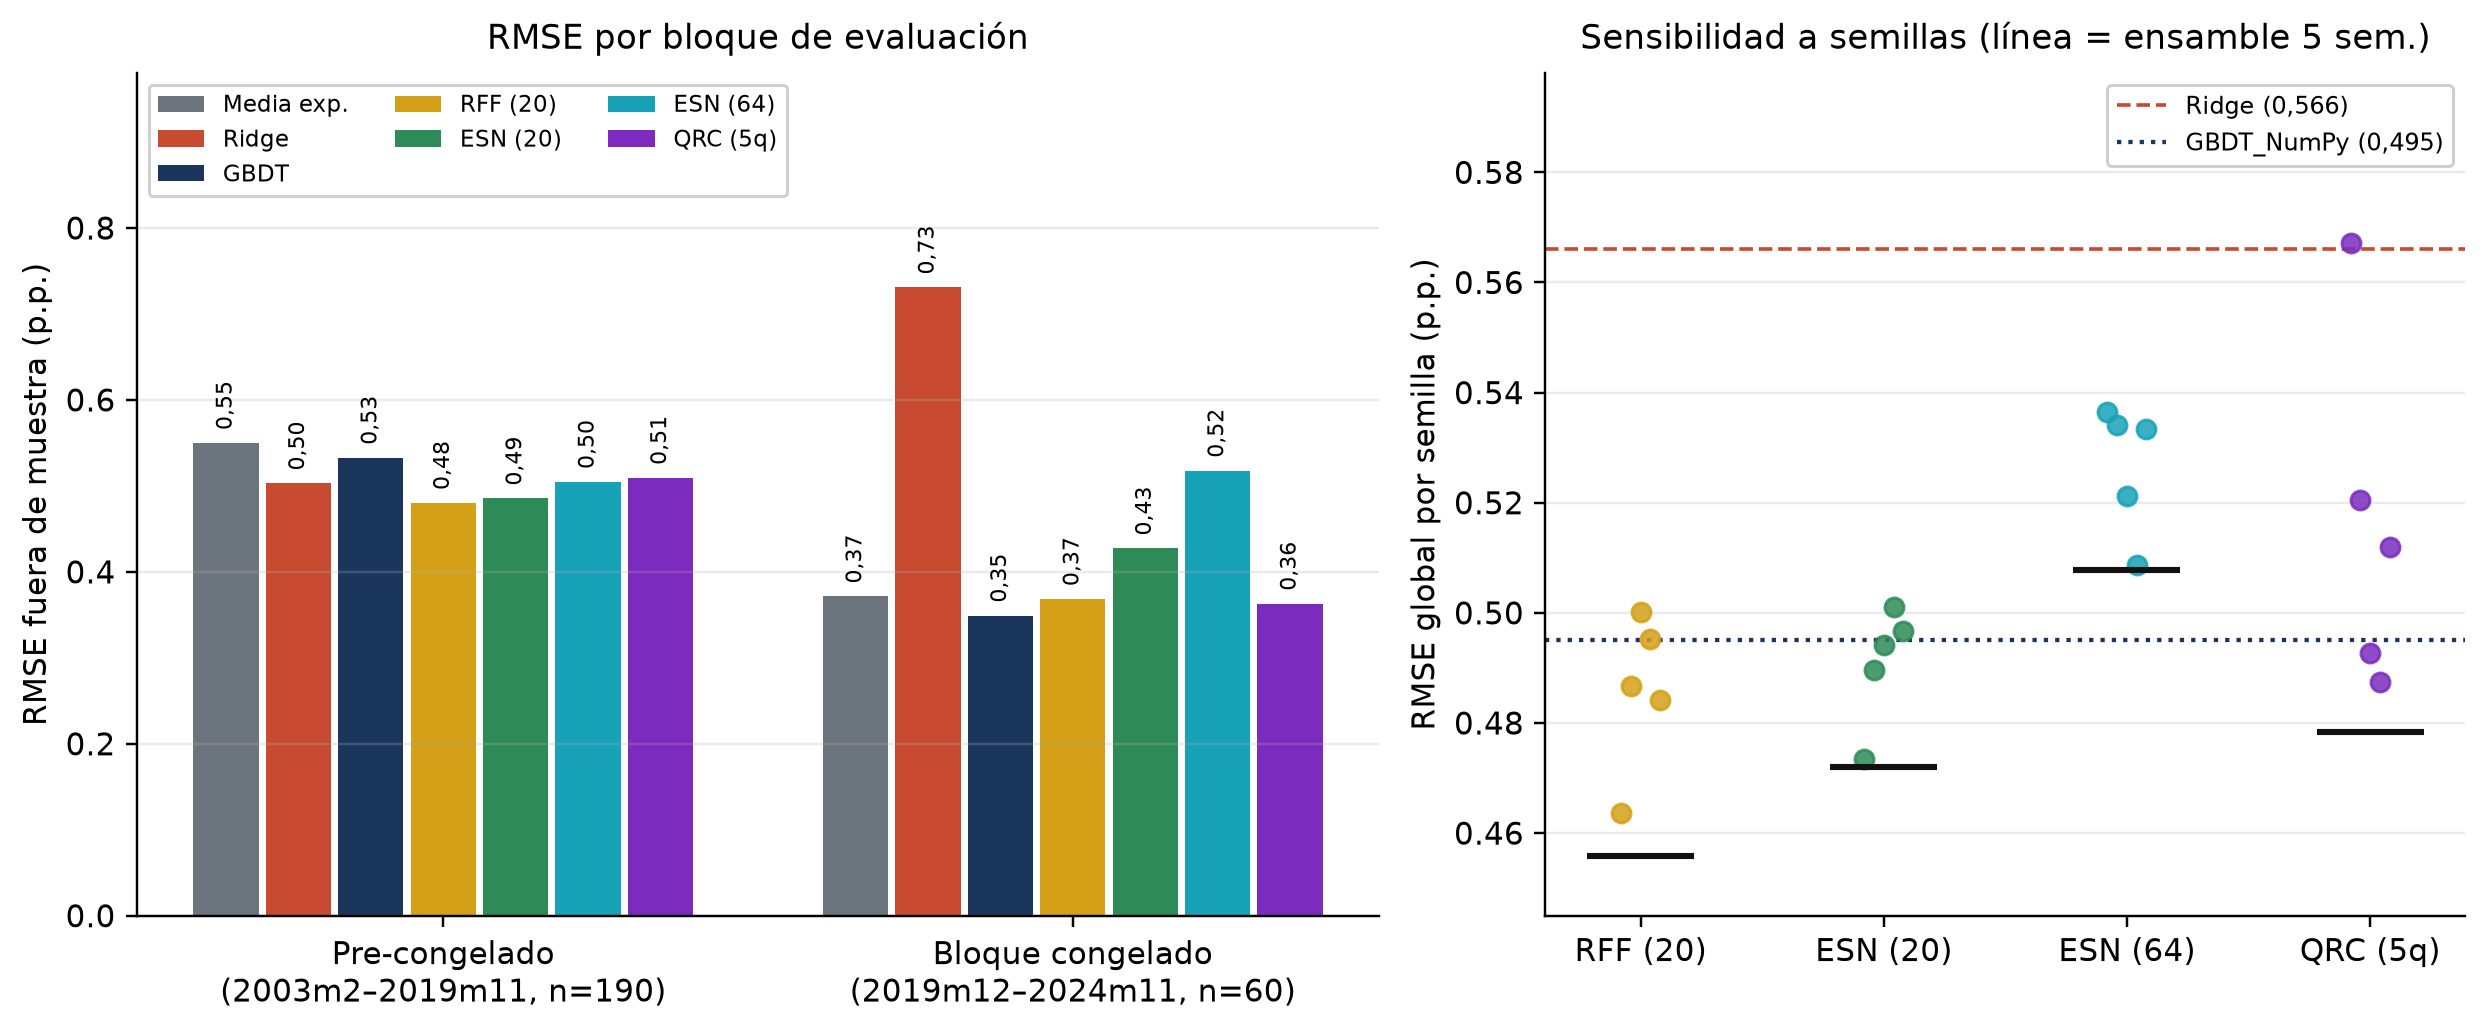
\includegraphics[width=0.96\textwidth]{images/etapa4_estabilidad_regimenes.png}
	\caption{Comparación de RMSE entre período pre-pandemia y tramo final (izquierda) y dispersión entre cinco semillas frente al promedio (derecha).}
	\label{fig:etapa4_estabilidad}
\end{figure}

\subsection{Qué muestran las simulaciones calibradas y cuánta ventaja es detectable}
\label{subsec:experimento_sintetico}

Como una serie histórica única de \(250\) meses puede ocultar situaciones favorables o desfavorables, se construyeron doce escenarios simulados inspirados en los parámetros reales del PBI peruano (\(300\) remuestreos de incertidumbre por bloques sobre \(n=314\) observaciones; Tabla~\ref{tab:etapa6_sintetico} y Figura~\ref{fig:etapa6_delta}). En cada escenario se ejecutaron veinte simulaciones midiendo la mejora porcentual de QRC respecto a cada competidor \(B\):
\[
\Delta_B(\theta)=
100\left(
\frac{\RMSE_{B}(\theta)-\RMSE_{\QRC}(\theta)}
{\RMSE_{B}(\theta)}
\right),
\]
considerando favorable un escenario (\(\theta \in \mathcal{A}\)) solo cuando la mejora superaba el \(2{,}0\%\) mínimo y su intervalo de confianza era positivo.

\begin{table}[htbp]
	\centering
	\caption{Simulaciones calibradas: error RMSE promedio, mejora relativa \(\Delta(\theta)\) de QRC y escenarios favorables (\(\delta_{\min}=2{,}0\%\))}
	\label{tab:etapa6_sintetico}
	\footnotesize
	\renewcommand{\arraystretch}{1.12}
	\begin{tabular}{@{}>{\raggedright\arraybackslash}p{3.9cm}S[table-format=1.3]S[table-format=1.3]S[table-format=1.3]S[table-format=1.3]S[table-format=-2.2]S[table-format=-2.2]c@{}}
		\toprule
		Escenario & {Ridge} & {RFF} & {ESN} & {QRC} & {\(\Delta_{\text{Ridge}}\) (\%)} & {\(\Delta_{\text{ESN}}\) (\%)} & {Favorable?}\\
		\midrule
		Calibrado Perú (\(T=350\)) & 0.606 & 0.617 & 0.620 & 0.652 & -7.49 & -5.08 & No\\
		Muestra mediana (\(T=700\)) & 0.619 & 0.629 & 0.638 & 0.669 & -8.53 & -5.29 & No\\
		Muestra larga (\(T=1400\)) & 0.642 & 0.649 & 0.662 & 0.695 & -8.42 & -5.06 & No\\
		Persistencia baja (\(\phi=0{,}10\)) & 0.640 & 0.642 & 0.645 & 0.647 & -1.32 & -0.45 & No\\
		Persistencia alta (\(\phi=0{,}65\)) & 0.664 & 0.701 & 0.724 & 0.801 & -20.90 & -11.16 & No\\
		Señal baja (\(0{,}5\times\)) & 0.655 & 0.665 & 0.669 & 0.680 & -3.62 & -1.32 & No\\
		Señal alta (\(2{,}5\times\)) & 0.638 & 0.652 & 0.665 & 0.705 & -11.62 & -6.67 & No\\
		Ruido normal sin cambios (\(T=350\)) & 0.630 & 0.646 & 0.649 & 0.672 & -6.39 & -3.45 & No\\
		No lineal + choques (\(T=350\)) & 0.615 & 0.621 & 0.620 & 0.634 & -2.99 & -2.13 & No\\
		No lineal + choques (\(T=1000\)) & 0.624 & 0.618 & 0.617 & 0.633 & -1.36 & -2.41 & No\\
		Pocas variables (\(d=2\)) & 0.622 & 0.631 & 0.631 & 0.656 & -5.87 & -4.05 & No\\
		Muchas variables (\(d=8\)) & 0.693 & 0.715 & 0.723 & 0.753 & -8.48 & -4.14 & No\\
		\bottomrule
	\end{tabular}
	\fuente{elaboración propia con base en las simulaciones calibradas del estudio (\(20\) repeticiones por escenario).}
\end{table}

Las conclusiones de los doce mundos simulados son consistentes:
\begin{enumerate}
	\item \textbf{Ningún escenario favoreció al modelo cuántico (\(\mathcal{A}=\emptyset\)):} QRC no ganó en ninguno de los doce casos probados, ni siquiera al aumentar el historial a \(1\,400\) meses (donde siguió \(8{,}4\%\) por detrás de Ridge). Esto confirma que en el Perú no venció a Ridge por mérito cuántico, sino porque la pandemia hizo fallar las rectas lineales y por promediar cinco semillas.
	\item \textbf{Donde hay memoria lineal fuerte, QRC pierde más:} cuando el patrón anual es intenso (\(\phi=0{,}65\)), transformar las variables en ángulos cuánticos distorsiona esa relación simple y QRC queda \(20{,}90\%\) por detrás de Ridge.
	\item \textbf{Con curvas y choques fuertes también ganan los modelos clásicos:} cuando la economía artificial incluye choques bruscos y \(1\,000\) meses, ESN (\(0{,}617\)) y RFF (\(0{,}618\)) superan a Ridge (\(0{,}624\)) y mantienen cerca de \(2{,}3\%\) de ventaja sobre QRC (\(0{,}633\)).
\end{enumerate}

Además, se calculó cuánta ventaja real haría falta en los \(250\) meses peruanos para que las pruebas estadísticas la detecten con seguridad al \(80\%\) (Figura~\ref{fig:etapa6_potencia} y Anexo~\ref{app:potencia}). Debido a la fuerte agitación de la pandemia, frente a Ridge se necesitaría una mejora enorme de \(36{,}1\%\) para probar ventaja con certeza; y frente a los controles clásicos más estables se necesitaría entre \(5{,}7\%\) (RFF), \(7{,}6\%\) (media histórica) y \(11{,}1\%\) (ESN). En otras palabras, con el tamaño actual de la serie peruana no es posible distinguir con seguridad mejoras pequeñas del orden del \(2\%\).

\begin{figure}[htbp]
	\centering
	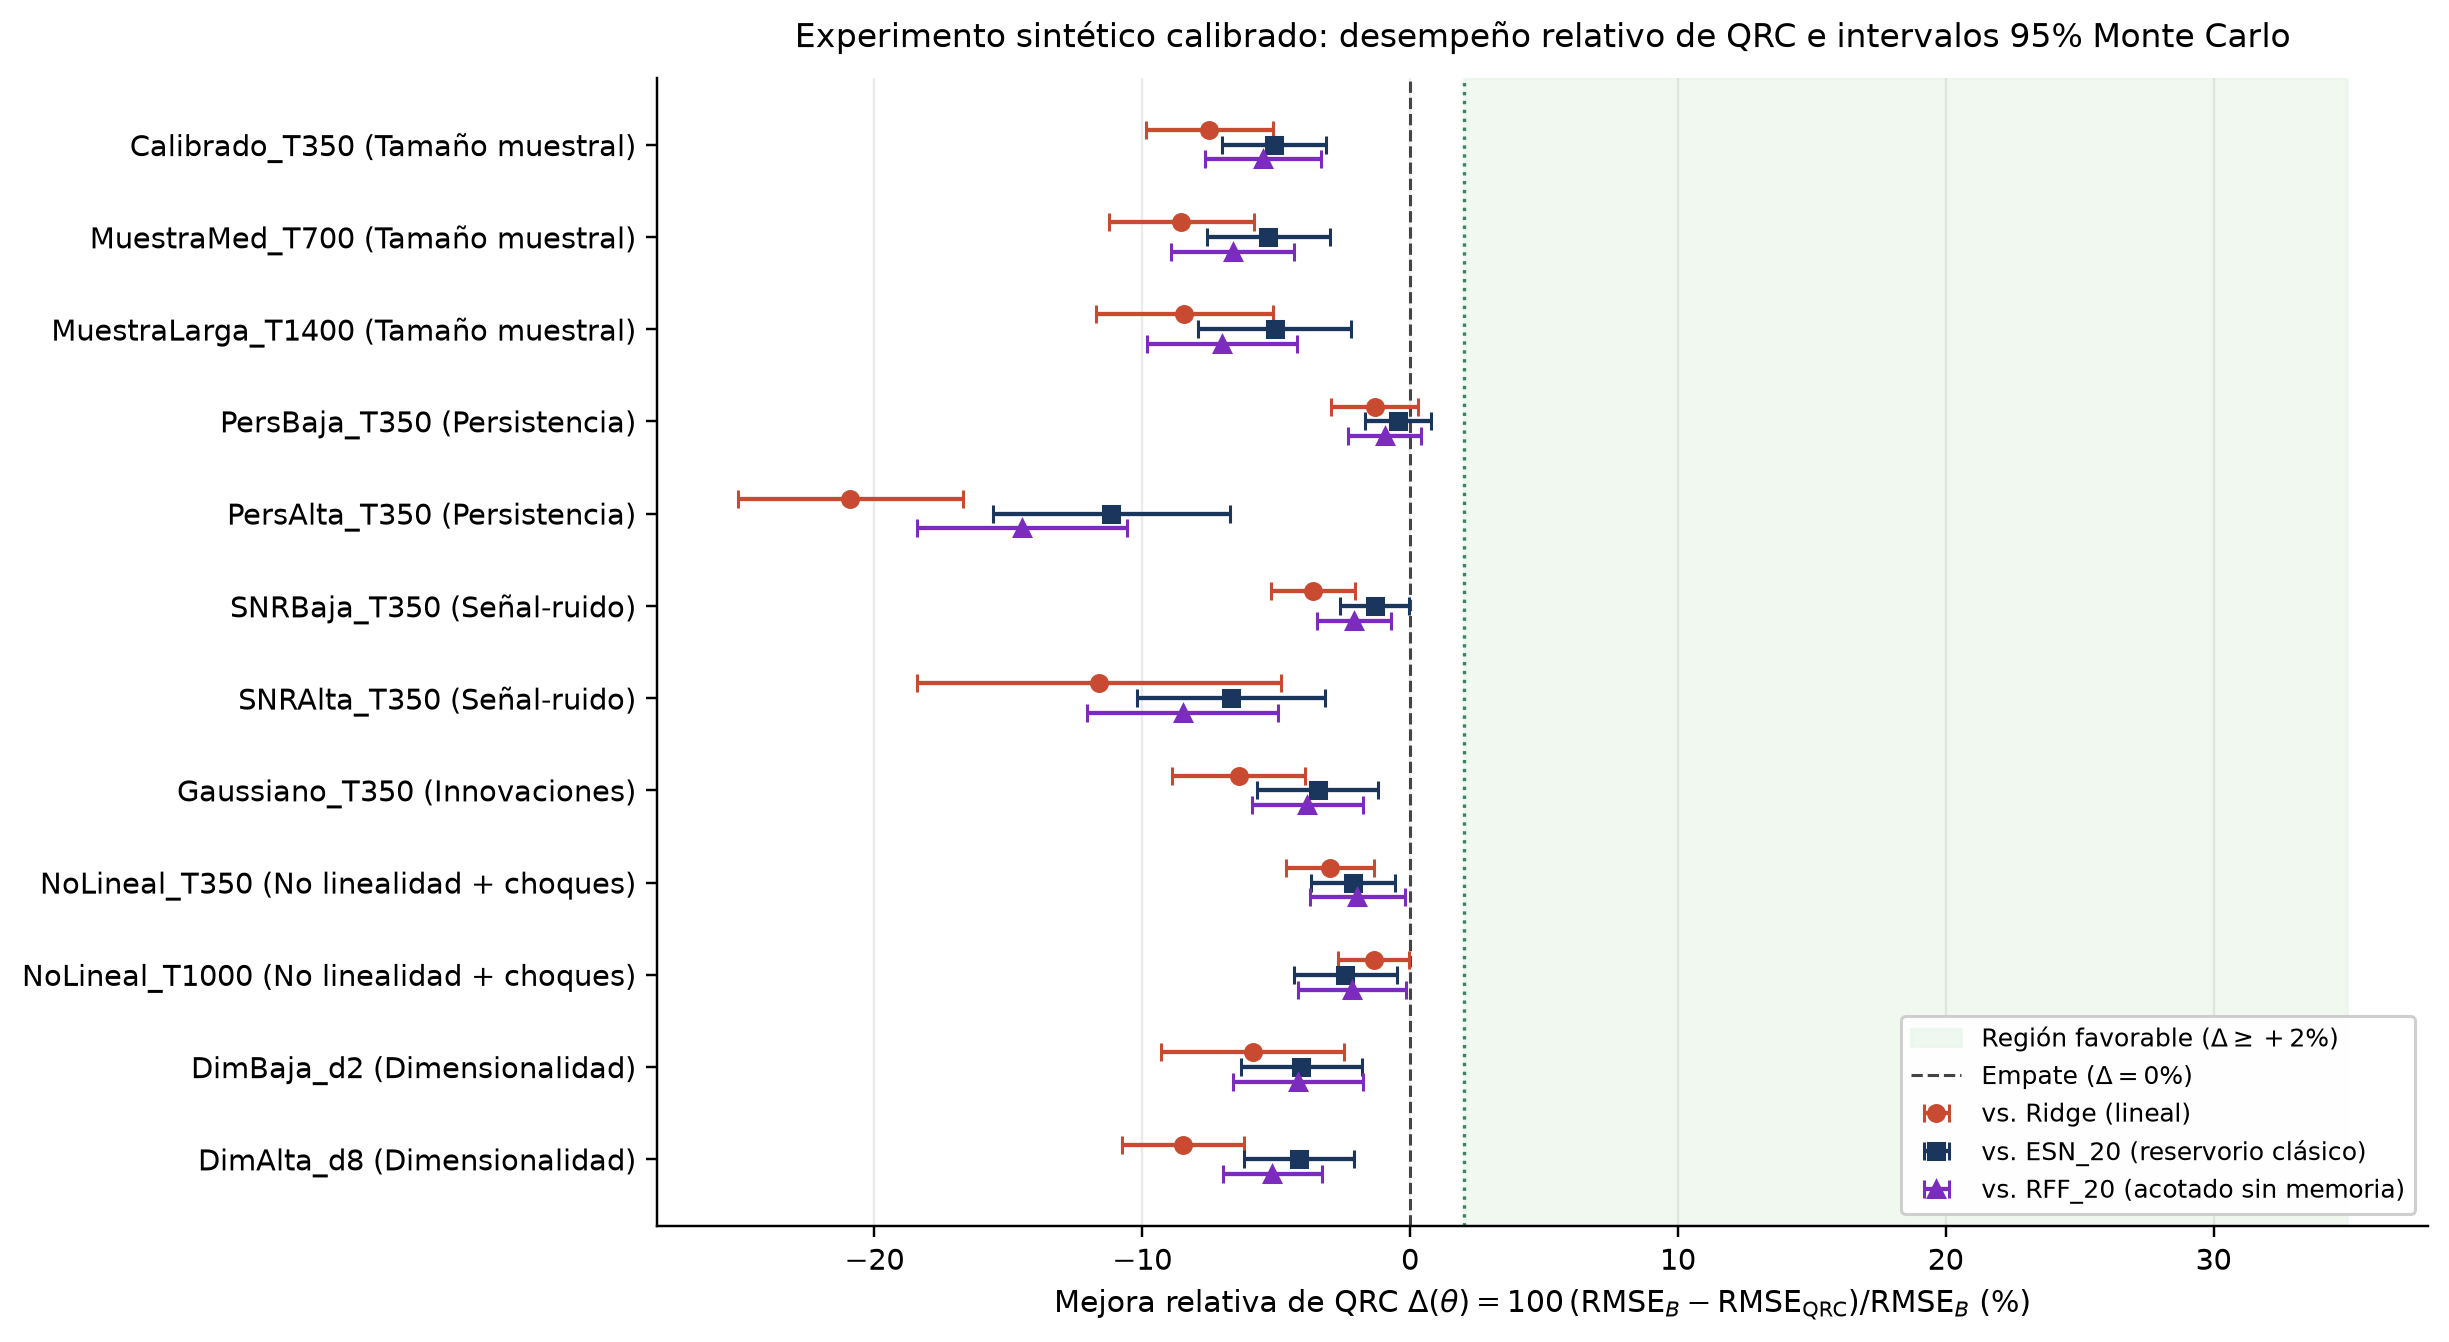
\includegraphics[width=0.96\textwidth]{images/etapa6_delta_escenarios.png}
	\caption{Diferencia porcentual relativa \(\Delta(\theta)\) de QRC e intervalos al 95\% en los doce escenarios simulados.}
	\label{fig:etapa6_delta}
\end{figure}

\begin{figure}[htbp]
	\centering
	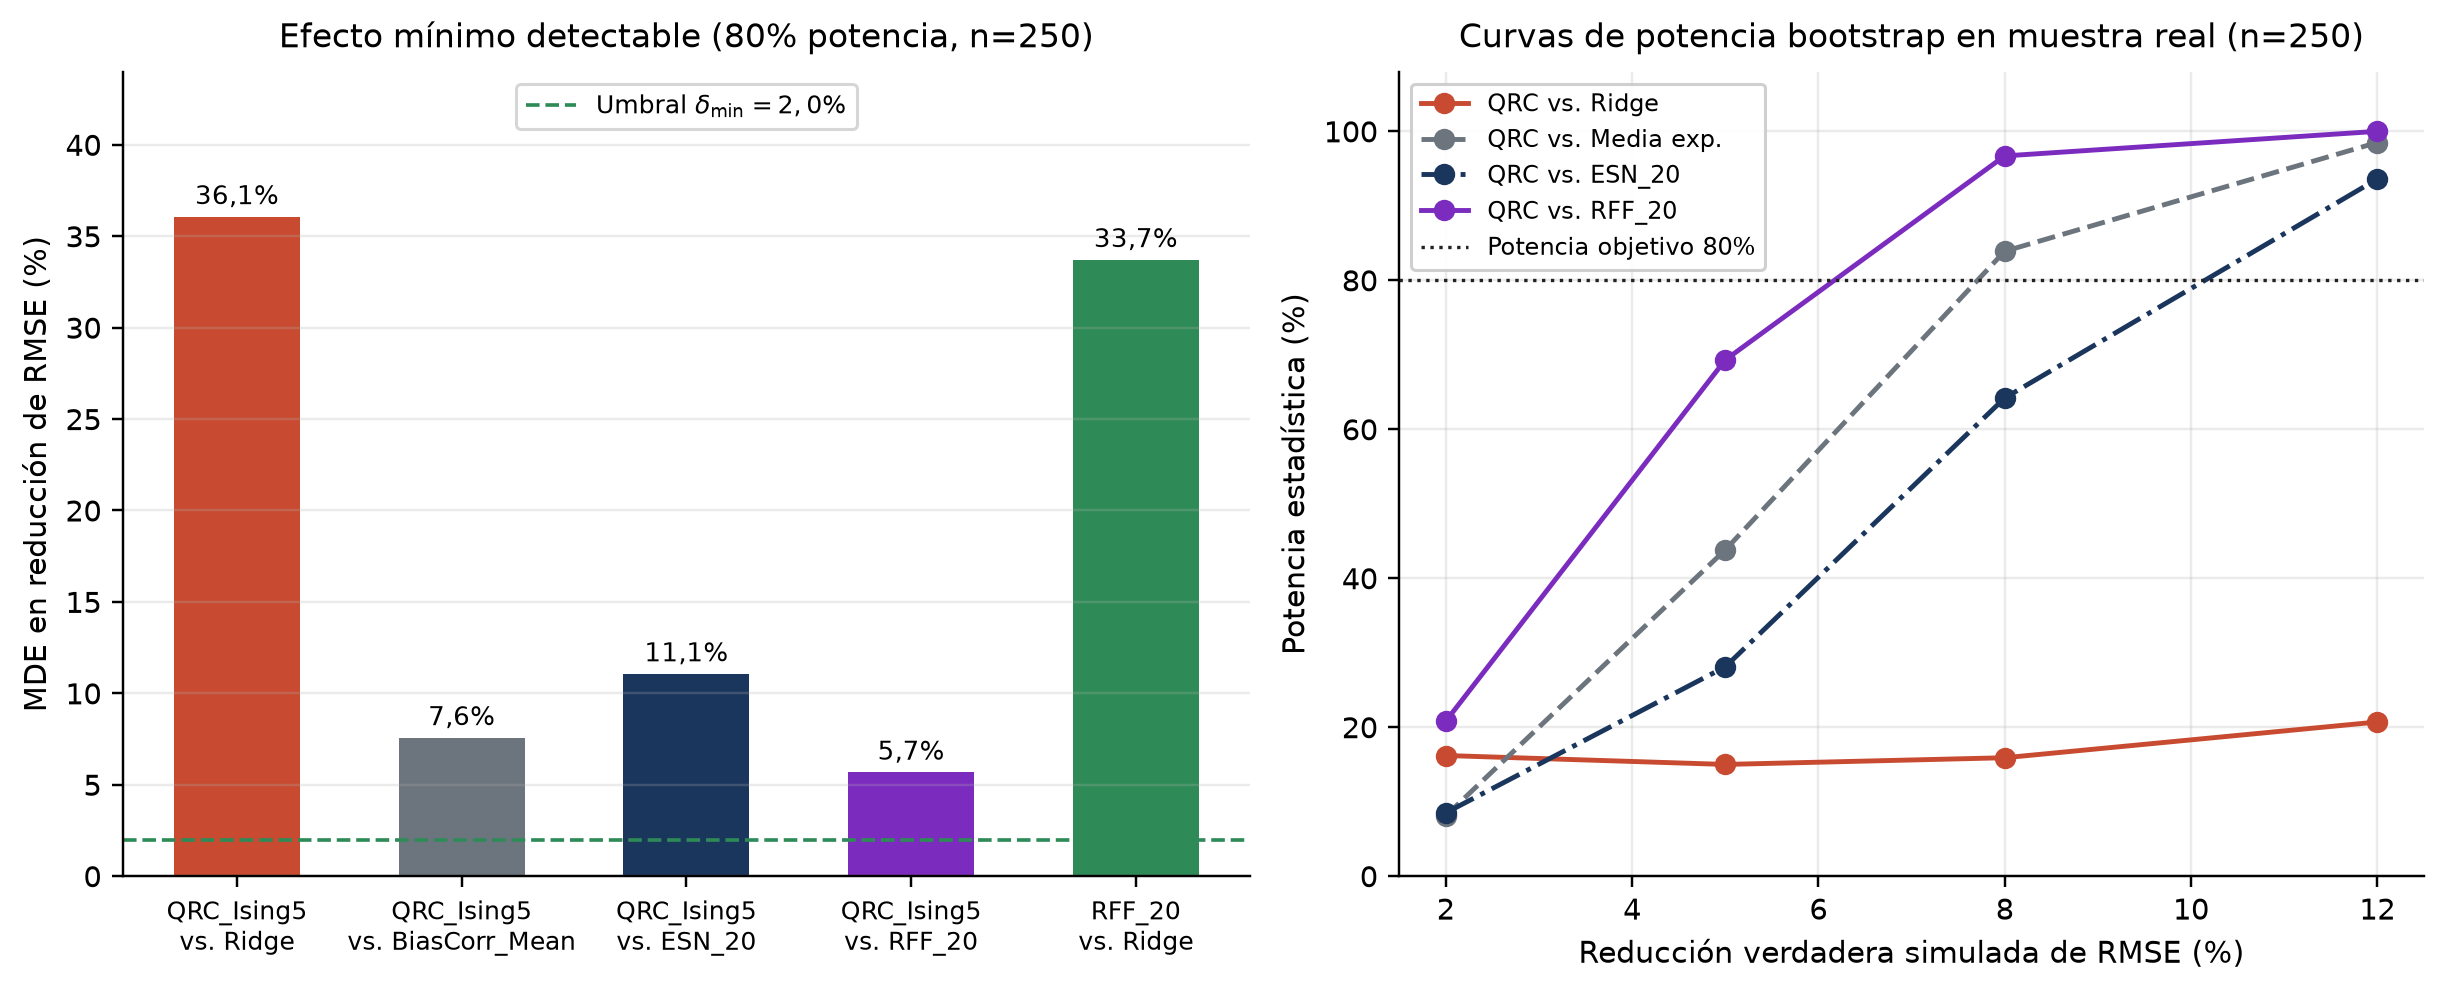
\includegraphics[width=0.96\textwidth]{images/etapa6_potencia_mde.png}
	\caption{Mejora mínima detectable con 80\% de seguridad (izquierda) y probabilidad de detección según tamaño real de ganancia en \(n=250\) orígenes (derecha).}
	\label{fig:etapa6_potencia}
\end{figure}

\subsection{Por qué no se realizó la evaluación económica}
\label{subsec:analisis_economico}

De acuerdo con la regla fijada desde el inicio (Anexo~\ref{app:voi}), solo se estimarían ganancias o pérdidas monetarias si QRC superaba de forma clara y robusta tanto a Ridge como a sus pares clásicos. Al no ganar ninguna comparación múltiple, quedar por detrás de RFF y no mostrar ventaja en las simulaciones (\(\mathcal{A}=\emptyset\)), la evaluación económica se detuvo para no atribuir beneficios económicos artificiales.

\subsection{Pruebas conjuntas finales para evitar falsos positivos}
\label{subsec:inferencia_integrada_etapa8}

Cuando se comparan varios modelos a la vez, algún resultado puede parecer significativo simplemente por suerte. Para evitarlo, la Tabla~\ref{tab:etapa8_holm} aplica correcciones por comparaciones múltiples \parencite{holm1979,benjamini1995} sobre los siete contrastes principales de QRC, y la Tabla~\ref{tab:etapa8_mcs} (junto con la Figura~\ref{fig:etapa8_mcs}) aplica el método del conjunto de confianza de modelos de \textcite{hansen2011}, que agrupa a todos los modelos que estadísticamente siguen empatados en precisión.

\begin{table}[htbp]
	\centering
	\caption{Comparaciones directas de QRC con ajuste por pruebas múltiples}
	\label{tab:etapa8_holm}
	\scriptsize
	\setlength{\tabcolsep}{3.5pt}
	\renewcommand{\arraystretch}{1.14}
	\begin{tabular}{@{}>{\raggedright\arraybackslash}p{3.1cm}S[table-format=1.3]S[table-format=-1.3]cS[table-format=1.4]S[table-format=1.4]S[table-format=1.4]>{\raggedright\arraybackslash}p{2.7cm}@{}}
		\toprule
		Comparador (\(n=250\)) & {\(\text{RMSE}\)} & {\(\Delta\)} & {\(\text{IC}_{95\%}\) boot.} & {\(p_{\text{DM}}\)} & {\(p_{\text{Holm}}\)} & {\(p_{\text{BH}}\)} & Resultado formal\\
		\midrule
		Referencia nula (\(\widehat{Y}=0\)) & 0.574 & -0.096 & \([-0{,}191;\, 0{,}002]\) & 0.1131 & 0.5656 & 0.2640 & Resultado inconcluso\\
		Corrección media exp. & 0.513 & -0.034 & \([-0{,}060;\, -0{,}010]\) & 0.0175 & 0.1052 & 0.0614 & Mejora sin sig. Holm\\
		Autorregresivo AR (BIC) & 0.498 & -0.020 & \([-0{,}057;\, 0{,}019]\) & 0.3811 & 0.8094 & 0.4447 & Resultado inconcluso\\
		Regresión Ridge & 0.566 & -0.088 & \([-0{,}208;\, 0{,}020]\) & 0.1957 & 0.7830 & 0.3426 & Resultado inconcluso\\
		Árboles potenciados (GBDT) & 0.495 & -0.017 & \([-0{,}044;\, 0{,}008]\) & 0.2698 & 0.8094 & 0.3777 & Resultado inconcluso\\
		ESN clásica (20 neuronas) & 0.472 & 0.006 & \([-0{,}032;\, 0{,}038]\) & 0.7296 & 0.8094 & 0.7296 & Resultado inconcluso\\
		Características aleatorias (RFF) & 0.456 & 0.022 & \([+0{,}006;\, +0{,}038]\) & 0.0146 & 0.1023 & 0.0614 & Desventaja sin sig. Holm\\
		\midrule
		\multicolumn{8}{@{}l}{\textit{Único contraste significativo tras Holm en los subperíodos (pre-pandemia \(n=190\)):}}\\
		Características RFF (pre-COVID) & 0.480 & 0.029 & \([+0{,}012;\, +0{,}046]\) & 0.0038 & 0.0265 & 0.0265 & Evidencia desfavorable\\
		\bottomrule
	\end{tabular}
	\fuente{elaboración propia a partir de las pruebas comparativas del estudio. \(\text{RMSE}_{\text{QRC}}=0{,}478\) en \(n=250\) y \(0{,}509\) en \(n=190\); \(\Delta=\text{RMSE}_{\text{QRC}}-\text{RMSE}_{\text{comp}}<0\) favorece a QRC.}
\end{table}

La Tabla~\ref{tab:etapa8_holm} deja dos certezas simples: primero, la pequeña ventaja puntual de QRC sobre el promedio histórico (\(p=0{,}0175\) aislado) pierde validez al corregir por comparaciones múltiples (\(p_{\text{Holm}}=0{,}1052\)); segundo, el único contraste firme tras corrección ocurre \textbf{en contra de QRC}, pues antes de la pandemia el método clásico RFF logra mayor precisión estadística (\(p_{\text{Holm}}=0{,}0265\)). En el bloque final de \(60\) meses todos los contrastes ajustados marcan empate estadístico (\(p_{\text{Holm}}=1{,}000\)).

\begin{table}[htbp]
	\centering
	\caption{Permanencia de los doce modelos dentro del grupo de mejores modelos empatados (\(p_{\text{MCS}}\))}
	\label{tab:etapa8_mcs}
	\footnotesize
	\setlength{\tabcolsep}{5.5pt}
	\renewcommand{\arraystretch}{1.12}
	\begin{tabular}{@{}>{\raggedright\arraybackslash}p{4.4cm}S[table-format=1.3]S[table-format=1.3]S[table-format=1.3]S[table-format=1.3]S[table-format=1.3]S[table-format=1.3]@{}}
		\toprule
		& \multicolumn{2}{c}{Global (\(n=250\))} & \multicolumn{2}{c}{Pre-pandemia (\(n=190\))} & \multicolumn{2}{c}{Tramo final (\(n=60\))}\\
		\cmidrule(lr){2-3} \cmidrule(lr){4-5} \cmidrule(lr){6-7}
		Modelo & {MSE} & {MAE} & {MSE} & {MAE} & {MSE} & {MAE}\\
		\midrule
		Características aleatorias (RFF) & 1.000 & 1.000 & 1.000 & 1.000 & 0.713 & 0.880\\
		Reservorio clásico ESN (20 n.) & 0.674 & 0.827 & 0.767 & 0.922 & 0.584 & 0.880\\
		Reservorio cuántico QRC (5 qubits) & 0.674 & 0.827 & 0.767 & 0.922 & 0.713 & 0.880\\
		Árboles potenciados (GBDT) & 0.674 & 0.827 & 0.549 & 0.708 & 1.000 & 1.000\\
		Autorregresivo AR (BIC) & 0.674 & 0.827 & 0.767 & 0.922 & 0.584 & 0.880\\
		Reservorio clásico ESN (64 n.) & 0.674 & 0.827 & 0.767 & 0.922 & 0.378 & 0.442\\
		Corrección de sesgo (media exp.) & 0.640 & 0.512 & 0.097 & 0.003 & 0.713 & 0.880\\
		Corrección de sesgo (móvil 60m) & 0.640 & 0.827 & 0.118 & 0.247 & 0.713 & 0.880\\
		ARX observable (BIC) & 0.640 & 0.827 & 0.549 & 0.922 & 0.346 & 0.442\\
		Regresión Ridge (benchmark) & 0.640 & 0.827 & 0.767 & 0.922 & 0.187 & 0.243\\
		Referencia nula (\(\widehat{Y}=0\)) & 0.640 & 0.827 & 0.549 & 0.922 & 0.353 & 0.442\\
		Factores dinámicos (DFM + Ridge) & 0.562 & 0.736 & 0.767 & 0.922 & 0.222 & 0.201\\
		\bottomrule
	\end{tabular}
	\fuente{elaboración propia a partir de la evaluación conjunta del estudio (\(T_{\max}\), \(B=2000\)). Se mantiene en el grupo ganador al 90\% si \(p_{\text{MCS}}\ge 0{,}10\) (y al 75\% si \(p_{\text{MCS}}\ge 0{,}25\)).}
\end{table}

El análisis conjunto de la Tabla~\ref{tab:etapa8_mcs} y la Figura~\ref{fig:etapa8_mcs} resume toda la evaluación:
\begin{itemize}
	\item \textbf{En toda la muestra (2003--2024):} ninguno de los doce modelos queda descartado definitivamente, aunque RFF ocupa el primer lugar (\(p_{\text{MCS}}=1{,}000\)) y ESN, QRC, AR y GBDT forman un grupo equivalente detrás.
	\item \textbf{Separando épocas normales y pandemia:} antes de 2020, el método descarta la simple corrección por promedio histórico (\(p=0{,}097\)); mientras que durante la pandemia, encabezan los árboles potenciados (\(p=1{,}000\)), seguidos de RFF y QRC (\(p=0{,}713\)), expulsando del grupo líder al 75\% a los modelos lineales no acotados (Ridge, \(p=0{,}187\); factores dinámicos, \(p=0{,}222\)).
\end{itemize}

\begin{figure}[htbp]
	\centering
	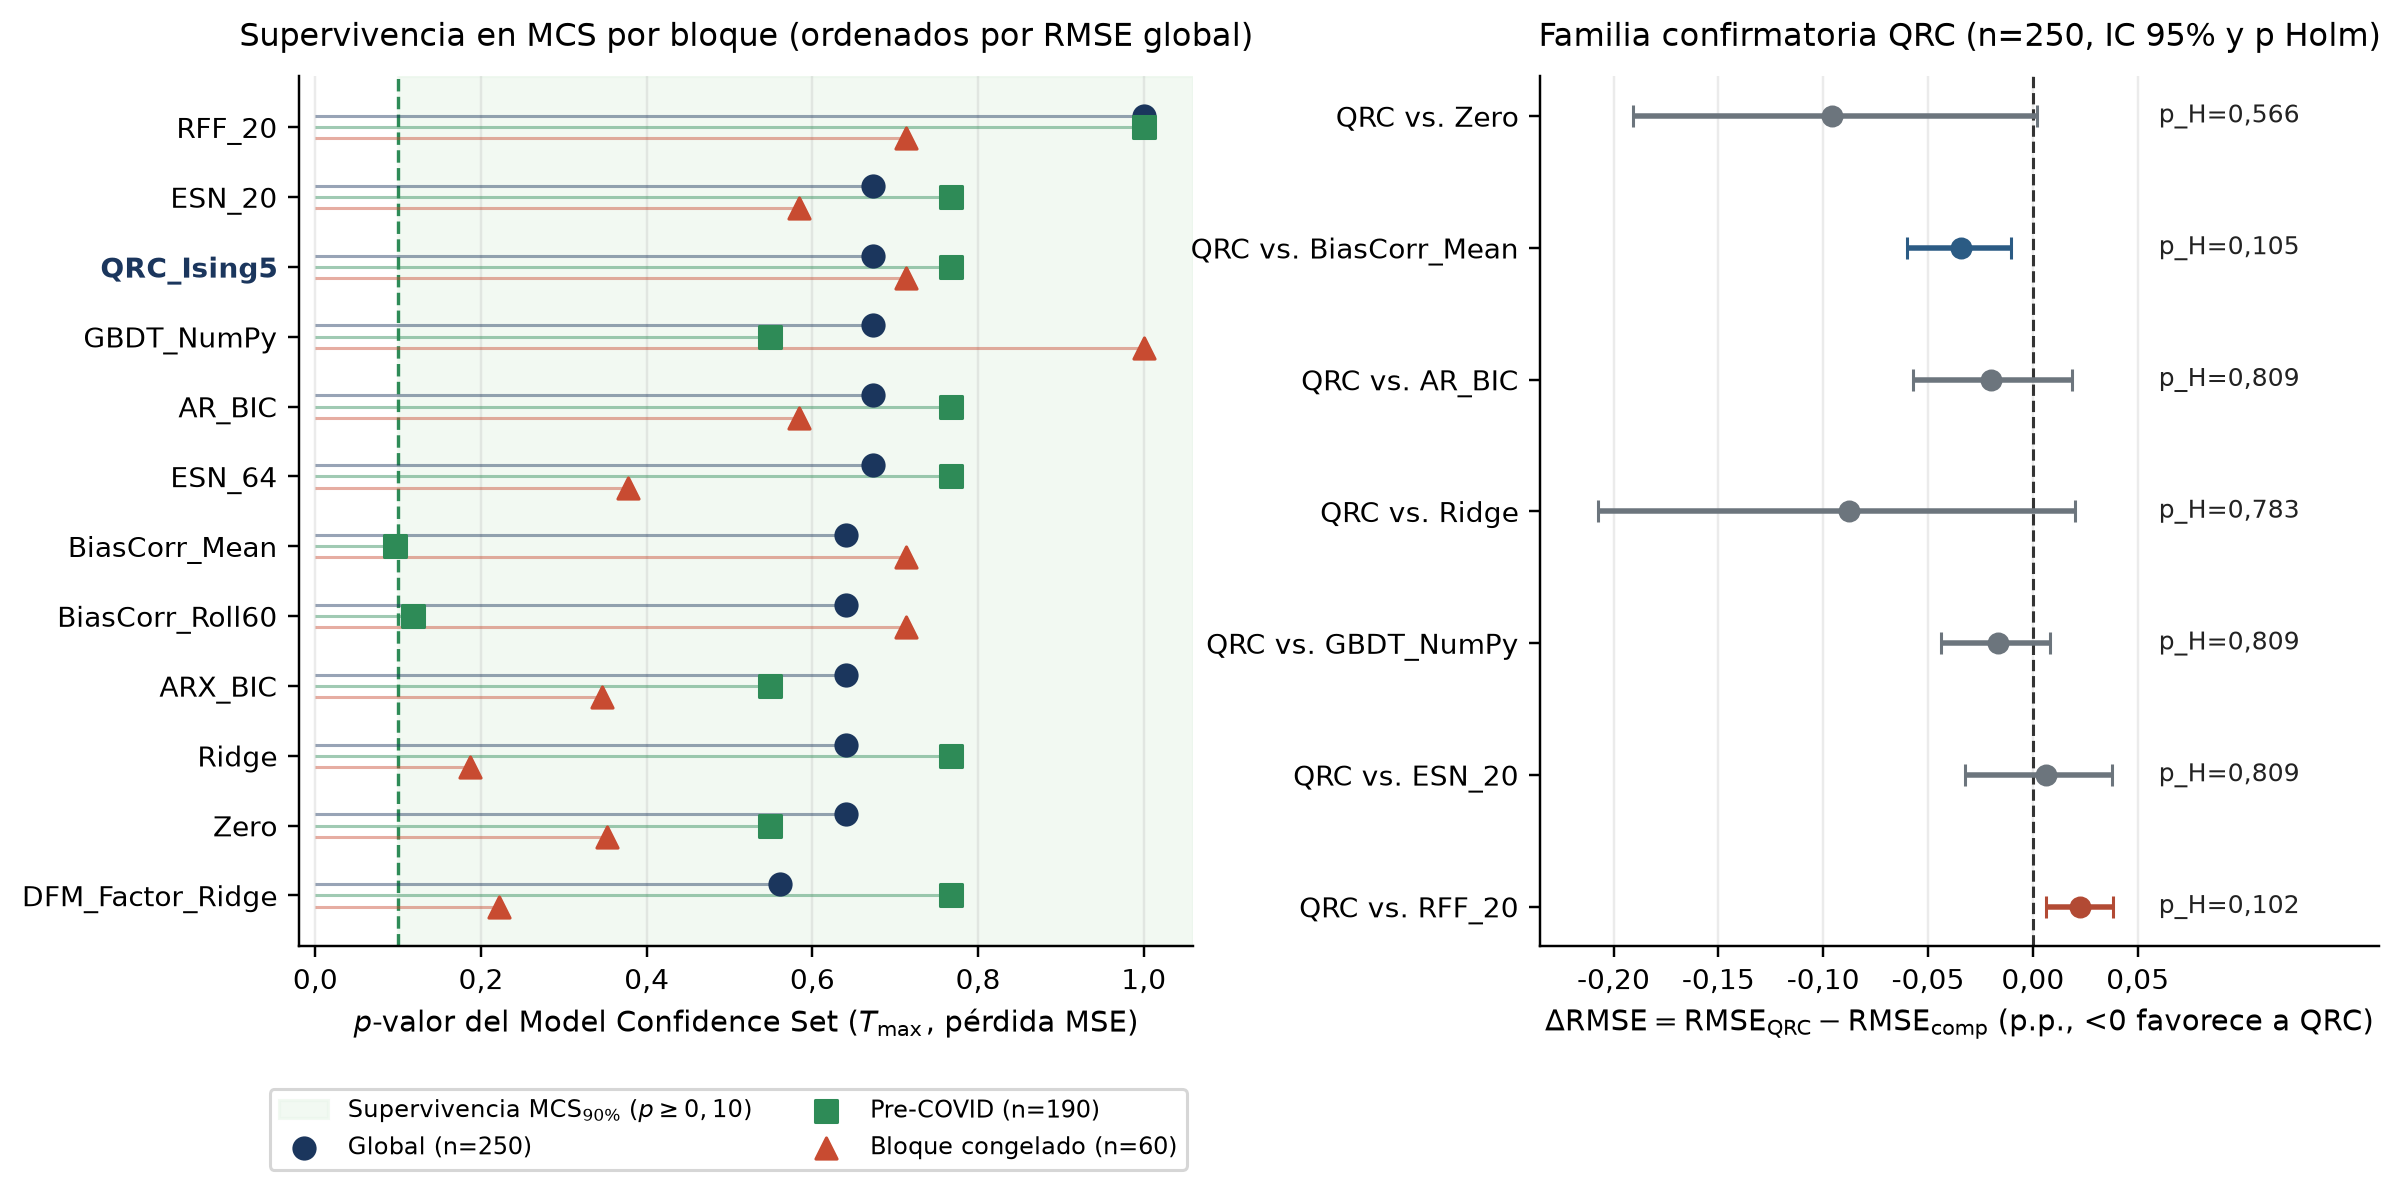
\includegraphics[width=0.98\textwidth]{images/etapa8_mcs_inferencia.png}
	\caption{Supervivencia en el grupo de mejores modelos por época (izquierda) y comparaciones directas de QRC en \(n=250\) con márgenes al 95\% (derecha).}
	\label{fig:etapa8_mcs}
\end{figure}
